%
% ---------------------------------------------------------------------------------------
% 2010 / 1.431E+20 POT Muon-Neutrino Disappearance Analysis (3-Flavour)
% ---------------------------------------------------------------------------------------
%

\documentclass[final]{elsarticle}

\usepackage[margin=2.00cm]{geometry}  % tweak margins
%\usepackage{draftcopy}                % uncomment to print a "DRAFT-COPY" in background
\usepackage{graphicx}                 % if you want to include PostScript figures
\usepackage[figuresright]{rotating}   % if you have landscape tables
\usepackage{multirow}                 % fancy tables
\usepackage[toc,page]{appendix}       % appendix
\usepackage{lineno}                   % for printing the line numbers
\usepackage{natbib}                   % for building bibliography with \cite{}
\usepackage{setspace}
\usepackage{times}
\usepackage{afterpage}
\usepackage{float}
\usepackage{subfigure}
\usepackage{color} 

% use to fix date
% \def \today { February 1st, 2009 }
% put your own definitions here:
\newcommand{\ttbs}{\char'134}
\newcommand{\AmS}{{\protect\the\textfont2
  A\kern-.1667em\lower.5ex\hbox{M}\kern-.125emS}}
% add words to TeX's hyphenation exception list
\hyphenation{author another created financial paper re-commend-ed Post-Script}

%\linenumbers
\bibliographystyle{elsart-num}

% By default, LaTeX doesn't like to fill more than 0.7 of a text page with tables and graphics, 
% nor does it like too many figures per page. Change this behaviour:
\renewcommand\floatpagefraction{.95}
\renewcommand\topfraction{.9}
\renewcommand\bottomfraction{.9}
\renewcommand\textfraction{.1}   
\setcounter{totalnumber}{50}
\setcounter{topnumber}{50}
\setcounter{bottomnumber}{50}


\begin{document}

% Title, authors, abstract and table of contents
%
% Front matter
%

\begin{frontmatter}

\title{
  T2K 1.431$\times10^{20}$-POT {\em 3-Flavour} Muon-Neutrino Disappearance Analysis
}

\vspace*{0.7cm}

\author[RAL]      {Costas Andreopoulos}
\author[RAL,OXF]  {Thomas Dealtry}
\author[VALENCIA] {Lorena Escudero S\'anchez}
\author[LANCS]    {and Nick Grant}

\address[RAL]{Particle Physics Dept., Rutherford Appleton Laboratory, STFC \\
              Harwell Science and Innovation Campus\\
              Oxfordshire OX11 0QX, UK}
\address[OXF]{Subdepartment of Particle Physics, University of Oxford \\
              Denys Wilkinson Building, Keble Road\\
              Oxfordshire OX1 3RH, UK}
\address[LANCS]{Physics Dept., Lancaster University \\
              Lancaster, LA1 4YB, UK}
\address[VALENCIA]{Instituto de Física Corpuscular, Edificio Institutos de Investigación \\
              Apartado de Correos 22085, E-46071 Valencia, Spain}

%
% Abstract
%

\begin{abstract}

We present the results of a 3-flavour $\nu_{\mu}$-disappearance analysis on the combined T2K Run 1+2 
dataset, which corresponds to an integrated J-PARC neutrino beam exposure of 1.431 $\times$ 10$^{20}$ POT. 
This analysis used 3-flavour oscillation probabilities instead of the 2-flavour approximation that was used 
in our earlier analysis reported in Ref.\ \cite{OurRun1and2Analysis2F}. Also oscillated $\nu_{e}$ templates 
were included in this analysis in the interaction modes CCQE, CC1$\pi$ and CC other, whereas these were 
neglected in the 2-flavour analysis. 

In the 3-flavour analysis, the total predicted number of single $\mu$-like ring events in Super-K is higher
for the inverted hierarchy (IH) than for the normal hierarchy (NH) if the atmospheric mass-squared difference
is $|\Delta m^{2}_{32}|$. This results from the prediction of more events above the oscillation maximum for 
the IH than for the NH and less below it, which is due to the 3-flavour $\nu_{\mu}$-survival probability being 
higher for the IH than the NH above the oscillation maximum and lower below the oscillation maximum. Since there 
are more events above the oscillation maximum than below it, the total predicted number is higher for the IH 
than for the NH. This is true for any combination of the non-23 oscillation parameters.

Uncertainties in $\delta_{CP}$ can change the predicted reconstructed spectrum of single $\mu$-like ring events
in Super-K by up to 5\% above the oscillation maximum and by up to 3\% below it. Meanwhile changes
in the spectrum due to uncertainties in $\sin^{2}(2 \theta_{13})$, $\sin^{2}(2 \theta_{12})$ and $\Delta m_{12}^{2}$ 
are relatively small at $\leq$ 0.5\%.

A 3-flavour $\nu_{\mu}$-disappearance fit was made of the observed Super-K reconstructed energy spectrum of
single $\mu$-like ring events in the combined Run 1+2 dataset. In this fit, sin$^{2}$(2$\theta_{23}$) and
$|\Delta m^{2}_{32}|$ were varied to find their best-fit values, but the non-23 oscillation parameters were
fixed. Using GENIE, this gave best-fit values of
sin$^{2}$(2$\theta_{23}$) = 0.98, $|\Delta m^{2}_{32}|$ = 2.6 $\times$ 10$^{-3}$ eV$^{2}$/c$^{4}$ for both mass
hierarchies, while a fit using NEUT gave sin$^{2}$(2$\theta_{23}$) = 0.99, $|\Delta m^{2}_{32}|$
= 2.6 $\times$ 10$^{-3}$ eV$^{2}$/c$^{4}$ for the NH and sin$^{2}$(2$\theta_{23}$) = 0.99, $|\Delta m^{2}_{32}|$
= 2.7 $\times$ 10$^{-3}$ eV$^{2}$/c$^{4}$ for the IH. For comparison, the best-fit values from the 2-flavour
analysis in \cite{OurRun1and2Analysis2F} were sin$^{2}$(2$\theta_{23}$) = 0.97, $|\Delta m^{2}_{32}|$
= 2.6 $\times$ 10$^{-3}$ eV$^{2}$/c$^{4}$ using GENIE and sin$^{2}$(2$\theta_{23}$) = 0.98, $|\Delta m^{2}_{32}|$
= 2.6 $\times$ 10$^{-3}$ eV$^{2}$/c$^{4}$ using NEUT. The 3-flavour best-fit points were higher in sin$^{2}$(2$\theta_{23}$)
than those in the 2-flavour analysis due to the effect of sin$^{2}$(2$\theta_{13}$): the 3-flavour analysis
used the value sin$^{2}$(2$\theta_{13}$) = 0.1, whereas the 2-flavour analysis used the approximation 
sin$^{2}$(2$\theta_{13}$) = 0.

Uncertainties in the best-fit points due to uncertainties in $\delta_{CP}$ were larger than those due to
uncertainties in $\sin^{2}(2 \theta_{13})$, $\sin^{2}(2 \theta_{12})$ and $\Delta m_{12}^{2}$; these uncertainties 
due to $\delta_{CP}$ were 0.5\% (NH) and 0.35\% (IH) in sin$^{2}$(2$\theta_{23}$) and 0.6\% (NH) and 0.4\% (IH) in
$|\Delta m^{2}_{32}|$. However this is relatively small compared with the combined systematic uncertainties in
the best-fit points which were 4.3 - 5.1\%.

The 3-flavour confidence contours are narrower in sin$^{2}$(2$\theta_{23}$) than the 2-flavour contours
since the 3-flavour best-fit points are nearer to sin$^{2}$(2$\theta_{23}$) = 1.0. The confidence contours
for the IH include higher values of $|\Delta m^{2}_{32}|$ than those for the NH; this is because it is necessary
to choose a higher value of this parameter for the IH than for the NH in order to fit the oscillation dip at a
certain energy in the real data.

\end{abstract}

%
% Keywords
%

%\begin{keyword}
%\end{keyword}

\end{frontmatter}

\clearpage

\tableofcontents

\clearpage

\listoffigures
\listoftables




% Main body
\clearpage

\section {Introduction }
\label{sec:intro}

In this note we present the results of a 3-flavour $\nu_{\mu}$-disappearance analysis on the combined T2K Run1+2
dataset. This work builds on the effective 2-flavour $\nu_{\mu}$-disappearance analysis of the Run1+2 dataset
that was reported in Ref.\ \cite{OurRun1and2Analysis2F}.
Further technical details of the effective 2-flavour analysis may be found in the analysis of the
Run 1 dataset that was reported in Ref.\ \cite{OurRun1DisappAnalysis2F}.

As the measurement error on the atmospheric $\Delta m^{2}$ 
approaches the solar $\Delta m^{2}$ ($\sim$0.075$\times$10$^{-3}$ eV$^2$/c$^{4}$),
subleading effects of the solar $\Delta m^{2}$ on $\nu_{\mu}$-disappearance analyses should not be neglected. 
This was pointed out by E.Lisi in the XIV International Workshop on Neutrino Telescopes \cite{LisiNeuTel11},
and brought to the attention of the T2K $\nu_{\mu}$-disappearance contour committee by M. Mezzetto.
In response, the contour committee recommended moving to a 3-flavour analysis \cite{T2KNuMuContourCom}.

The method for predicting the nominal Super-K reconstructed energy spectrum of single $\mu$-like ring events 
is described in Ref.\ \cite{OurRun1and2Analysis2F} and it is unchanged.
This work considers the same systematic uncertainties as Ref.\ \cite{OurRun1and2Analysis2F}.
As in the effective 2-flavour analysis, the best-fit oscillation parameters were found using the likelihood-ratio method \cite{StatAnalysisCowan}, 
and the confidence regions were constructed using the Feldman-Cousins method \cite{FeldmanCousins}.
Systematic errors were included in the oscillation contours using the Cousins-Highland method (Bayesian integration) 
and by determining their effects on the Feldman-Cousins $\Delta\chi^{2}_{critical}$ values.

The oscillation probabilities in this work were calculated in a full 3-flavour framework including matter effects. 
The $\nu_{\mu}$-survival probability depends on sin$^{2}$2$\theta_{12}$, sin$^{2}$2$\theta_{13}$, $\Delta m^{2}_{12}$, $\delta_{CP}$ 
and the neutrino mass hierarchy as well as sin$^{2}$2$\theta_{23}$ and $|\Delta m^{2}_{32}|$. Throughout this note $\sin^{2}(2 \theta_{12})$, 
$\sin^{2}(2 \theta_{13})$, $\Delta m_{21}^{2}$, $\delta_{CP}$ will be collectively denoted the ``non-23'' oscillation parameters. The method of 
calculation of the 3-flavour oscillation probabilities is described in Sec.\ \ref{sec:nuosc3f}, and details of the validation of the code and our 
assessment of the its numerical accuracy are also presented. The predicted reconstructed single $\mu$-like ring spectra in 
Super-K for the 3-flavour analysis are shown in Sec. \ref{sec:pred}. Details of the 3-flavour fits of toy MC datasets are given in 
Sec. \ref{sec:fits}; in this analysis, sin$^{2}$2$\theta_{12}$, sin$^{2}$2$\theta_{13}$, $\Delta m^{2}_{21}$ and $\delta_{CP}$ were 
randomised when creating the toy MC datasets but were fixed when fitting them or the real data. This section also includes the results of the 3-flavour 
fit of the Run1+2 dataset for both GENIE and NEUT, and a comparison with the results of the 2-flavour analysis \cite{OurRun1and2Analysis2F}. 
The 3-flavour confidence regions are shown in Sec.\ \ref{sec:conf_regions}, and these are compared with those obtained 
in the 2-flavour analysis \cite{OurRun1and2Analysis2F} and with previous results from MINOS \cite{Minos2011} and Super-K \cite{OldDisappSuperK}. 
A summary is given in Sec.\ \ref{sec:summary}.  



\section{3-flavour neutrino oscillation probabilities}
\label{sec:nuosc3f}

In this analysis, 3-flavour neutrino oscillation probabilities in constant density matter are used. Vacuum 3-flavour oscillation 
probabilites are also calculated, but these are used only to estimate the accuracy of the 3-flavour probabilities in matter (see 
section \ref{3flavouraccuracy}). 
The method of calculation of the vacuum probabilities is given in section \ref{vacuumosc}, while the calculation 
of the probabilities in constant density matter is described in section \ref{matterosc}. The code that makes these calculations 
has been integrated into the Rutherford/Oxford/Lancaster oscillation analysis package. In section \ref{3flavourresults}, 
comparisons are given between 2-flavour and 3-flavour (in matter) oscillation probabilities, and between 3-flavour oscillation probabilities 
in vacuum and matter. Validation of the code is described in section \ref{3flavourvalidation}: the vacuum probabilities were validated 
by comparing their values with those obtained from an alternative formulation in the PDG review. Several validation checks of 
the probabilities in constant density matter are made as they are calculated, and the values of the probabilities were checked 
by comparing them with those given by an independently-written program. Finally, an estimate of the accuracy of the oscillation 
probabilities in matter is given in section \ref{3flavouraccuracy}.
   
\subsection{3-flavour neutrino oscillation probabilities in vacuum}
\label{vacuumosc}

The 3-flavour neutrino oscillation probabilities in vacuum are calculated from equation 11 in \cite{kayser2005}:
\begin{equation}
P(\nu_{\alpha} \rightarrow \nu_{\beta}) = \delta_{\alpha \beta} - 4 \sum_{i>j} Re(U_{\alpha i}^{*} U_{\beta i} U_{\alpha j} U_{\beta j}^{*})
\sin^{2} \left( \frac{\Delta m_{ij}^{2} L}{4E} \right) + 2 \sum_{i>j} Im(U_{\alpha i}^{*} U_{\beta i} U_{\alpha j} U_{\beta j}^{*})
\sin \left(\frac{\Delta m_{ij}^{2} L}{2E} \right)
\label{3flavouroscprobvacuum}
\end{equation}
In equation \ref{3flavouroscprobvacuum}, $\Delta m_{ij}^{2}$ = $m_{j}^{2}$ - $m_{i}^{2}$, L is the distance from the neutrino target 
in Tokai to Super-K (295 km), E is the neutrino energy, and U is the PMNS matrix in vacuum:

\begin{equation}
U = \left(
\begin{array}{ccc}
c_{12}c_{13} & c_{13}s_{12} & s_{13}e^{-i\delta} \\
-c_{23}s_{12} - s_{13}s_{23}c_{12}e^{i\delta} & c_{12}c_{23} - s_{12}s_{13}s_{23}e^{i\delta} & c_{13}s_{23} \\
s_{12}s_{23} - s_{13}c_{12}c_{23}e^{i\delta} & -s_{23}c_{12} - s_{12}c_{23}s_{13}e^{i\delta} & c_{13}c_{23}
\end{array} \right)
\label{PMNSmatrix}
\end{equation}
with $s_{12} = \sin(\theta_{12})$, $c_{12} = \cos(\theta_{12})$, etc. $P(\bar{\nu}_{\alpha} \rightarrow \bar{\nu}_{\beta})$ 
is calculated by changing the sign of the third term in equation \ref{3flavouroscprobvacuum} (this assumes that CPT is 
conserved).

\subsection{3-flavour neutrino oscillation probabilities in constant density matter}
\label{matterosc}
All three neutrino flavours undergo neutral-current interactions with protons, neutrons and electrons in matter. These 
neutral-current interactions have identical amplitudes for all three flavours, and they produce no observable effects on
the probabilities of oscillation between one flavour and another. However the oscillation probabilities are changed by 
coherent forward scattering of electron neutrinos in charged-current interactions with electrons in matter \cite{kayser2005}.

Using natural units with $\hbar$ = c = 1, the time evolution of neutrino flavour states in vacuum is described by the 
Schr\"odinger equation:

\begin{equation}
i \frac{\partial \mathbf{\psi}}{\partial t} = H_{F} \mathbf{\psi} 
\end{equation}
where
\begin{equation}
  \mathbf{\psi} =\left(
\begin{array}{c}
\psi_{e} \\
\psi_{\mu} \\
\psi_{\tau}
\end{array} \right)
\end{equation}
and $H_{F}$ is the effective Hamiltonian in the flavour-state basis
\begin{equation}
H_{F} = \frac{1}{2E} U M U^{\dagger}
\end{equation}
with M defined by
\begin{equation}
M = \left(
\begin{array}{ccc}
0 & 0 & 0 \\
0 & \Delta m_{21}^{2} & 0 \\
0 & 0 & \Delta m_{31}^{2}
\end{array} \right)
\end{equation}
The calculation of oscillation probabilities requires neutrino flight time to be converted to distance travelled, 
and this conversion assumes that neutrinos are highly relativistic. In 
this calculation, $U M U^{\dagger}$ is used for neutrinos, but its complex conjugate is used for antineutrinos. For neutrinos, 
the effects of the charged-current interactions between electron neutrinos and electrons are taken into account by adding the 
potential $2E \sqrt{2} G_{F} N_{e}$ to the real part of the first diagonal element of $U M U^{\dagger}$, where E is the 
neutrino energy, $G_{F}$ is the Fermi coupling constant, and $N_{e}$ is the number density of electrons in matter. For 
antineutrinos, this potential is subtracted from the real part of the first diagonal element of the complex conjugate of 
$U M U^{\dagger}$ (for further details see section 9.2 in \cite{giunti}). 

After the addition or subtraction of this potential, $U M U^{\dagger}$ (or its complex conjugate) is diagonalised. The eigenvalues 
of a Hermitian matrix are always real; they are calculated by solving the (cubic) characteristic equation using the method 
of del Ferro, Tartaglia and Cardano as described in \cite{kopp}. The differences between the eigenvalues are the effective 
mass-squared differences in matter. The eigenvectors are calculated using an algebraic method: one of the components is set 
to be 1.0 (real), and the other two components are calculated using two of the three simultaneous equations in 
$U M U^{\dagger} - \lambda I = 0$, where the $\lambda$ are the eigenvalues. After being normalised, the three eigenvectors 
become the columns of the effective mixing matrix in matter. 

The initial flavour state of the neutrino is represented by a 1$\times$3 column vector whose entries are complex; if, for 
example, the initial flavour state is a muon neutrino, this column vector is 

\begin{displaymath}
\left(
\begin{array}{c}
0 \\
1 \\
0 
\end{array} \right)
\end{displaymath}
The vector representing the initial flavour state is then multiplied by the Hermitian conjugate of the matter mixing matrix 
to convert it to another 1$\times$3 complex column vector representing the initial mass states. These mass states are propagated 
to Super-K by multiplying the jth initial mass state by $\exp \left(\frac{-i \Delta m_{j1}^{2}L}{2E} \right)$, where the 
$\Delta m_{j1}^{2}$ are the mass-squared differences in matter, i.e.\ the differences between the eigenvalues of $U M U^{\dagger}$. 
This gives a new 1$\times$3 complex column vector representing the final mass states, and these are converted to the final flavour 
states by multiplying by the matter mixing matrix. The entries of the resulting 1$\times$3 complex column vector represent the 
amplitudes of each flavour at Super-K, and the corresponding oscillation probabilities are calculated as the moduli squared of these 
amplitudes.  

\subsection{Inputs to the 3-flavour neutrino oscillation probability calculations}

When calculating the 3-flavour oscillation probabilities, the mixing angles can be input either in the form $\sin^{2}(2 \theta_{ij})$ 
or as $\sin^{2}(\theta_{ij})$. $\sin(\theta_{ij})$ and $\cos(\theta_{ij})$ are calculated from the input values, and these are used in 
turn to calculate the elements of $U$. The ``solar'' mass-squared difference is input as $\Delta m_{21}^{2}$, and this is $>$ 0 for 
both mass hierarchies. The ``atmospheric'' 
mass-squared difference is input either as $|\Delta m_{32}^{2}|$ or using a definition introduced by G.\ Fogli, E.\ Lisi et al.\ in 
\cite{LisiGlobalAnalysis}:
\begin{equation}
\Delta m^{2}_{FL} = m_{3}^{2} - \frac{m_{2}^{2} + m_{1}^{2}}{2}
\end{equation}
The quantity denoted $\Delta m^{2}_{FL}$ is useful since its absolute value is the same for both mass hierarchies, and only its sign 
changes. If the atmospheric mass-squared difference is input as $\Delta m^{2}_{32}$, the mass hierarchy is set using the sign of 
$\Delta m_{32}^{2}$; this is positive for the normal mass hierarchy (NH) and negative for the inverted mass hierarchy (IH). In this case, 
$\Delta m_{31}^{2}$ is not input but is calculated as $\Delta m_{31}^{2}$ = $\Delta m_{21}^{2}$ + $\Delta m_{32}^{2}$ for both hierarchies.
If the atmospheric mass-squared difference is input as $\Delta m^{2}_{FL}$, the mass hierarchy is set using the sign of $\Delta m^{2}_{FL}$. 
Then $\Delta m_{32}^{2}$ and $\Delta m_{31}^{2}$ are calculated from the input values of $\Delta m^{2}_{FL}$ and $\Delta m_{21}^{2}$.

\subsection{Results of the 3-flavour neutrino oscillation probability calculations}
\label{3flavourresults}

A comparison of 2-flavour and 3-flavour (in matter) $\nu_{\mu}$-survival probabilities is given in figure \ref{pnumunumucomp}. 
In this figure, the nominal probabilities are calculated with $\sin^{2}(2 \theta_{12})$ = 0.87, $\sin^{2}(2 \theta_{13})$ = 0.1,
$\sin^{2}(2 \theta_{23})$ = 1.0, $\Delta m_{21}^{2}$ = 7.6 $\times 10^{-5}$  eV$^{2}$/c$^{4}$, $|\Delta m_{32}^{2}|$ = 2.32 $\times$ 10$^{-3}$ eV$^{2}$/c$^{4}$,
$\delta_{CP}$ = 0 and Earth crust density = 2.6 g/cm$^{3}$. The bands represent the maximum and minimum 3-flavour probabilities from 4000 random
variations of the non-23 oscillation parameters within their uncertainties at each energy with the same values of $\sin^{2}(2 \theta_{23})$ and
$|\Delta m_{32}^{2}|$ being used. The uncertainties in $\sin^{2}(2 \theta_{12})$ and $\Delta m_{21}^{2}$ are taken from KamLAND combined
with solar experiments \cite{Kamland}, while those in $\sin^{2}(2 \theta_{13})$ are computed as a weighted average of measurements from Daya Bay
\cite{DayaBay} and Reno \cite{Reno}.

The effect of $\sin^{2}(2 \theta_{13})$ on the 3-flavour $\nu_{\mu}$-survival probability in matter 
is shown in figure \ref{pnumunumus13}: there is a small increase in P($\nu_{\mu} \rightarrow \nu_{\mu}$) at all energies as 
$\sin^{2}(2 \theta_{13})$ increases. Also shown in figure \ref{pnumunumudelta} is the effect of $\delta_{CP}$ on the 3-flavour $\nu_{\mu}$-survival 
probability in matter: as $\delta_{CP}$ increases from 0 to $\pi$, P($\nu_{\mu}\rightarrow\nu_{\mu}$) increases above the oscillation 
maximum and decreases below it for the NH, with these changes being reversed for the IH. 
%A similar comparison for P($\nu_{\mu} \rightarrow \nu_{e}$) in matter is given in figure \ref{pnumunuecomp}, and the effect of $\delta_{CP}$ on
%P($\nu_{\mu} \rightarrow \nu_{e}$) in matter is given in figure \ref{pnumunuedelta}. 
The effects of uncertainties in $\sin^{2}(2 \theta_{12})$ and $\Delta m_{21}^{2}$ on the 3-flavour P($\nu_{\mu}\rightarrow\nu_{\mu}$) in matter 
are shown for the NH in table \ref{numuSurvProbEffectError12}. At 0.6 GeV, uncertainties in $\sin^{2}(2 \theta_{12})$ change 
P($\nu_{\mu}\rightarrow\nu_{\mu}$) by $\approx$ 0.00025 and uncertainties in $\Delta m_{21}^{2}$ change it by $\approx$ 0.0001. 

For the NH, the 3-flavour P($\nu_{\mu}\rightarrow\nu_{\mu}$) is increased below the oscillation
maximum and decreased above it compared with the 2-flavour probability, while for the IH these changes are reversed. The oscillation maximum is at
lower energy for the IH than for the NH, and this can be understood more easily by considering the vacuum probabilities. In equation 
\ref{3flavouroscprobvacuum}, the imaginary terms are zero if $\alpha$ = $\beta$, and only the 3 real terms contribute to the vacuum P($\nu_{\mu} \rightarrow \nu_{\mu}$). 
If the atmospheric mass-squared difference is input as $\Delta m^{2}_{32}$, the terms $|U_{\mu 1}|^{2}$, $|U_{\mu 2}|^{2}$, $|U_{\mu 3}|^{2}$, 
$sin^{2} \left( \frac{\Delta m_{21}^{2} L}{4E} \right)$ and sin$^{2} \left( \frac{\Delta m_{32}^{2} L}{4E} \right)$ are identical for the two hierarchies, 
and the only term that changes between them is sin$^{2} \left( \frac{\Delta m_{31}^{2} L}{4E} \right)$. Since $\Delta m_{31}^{2}$ is lower for the 
IH than for the NH, sin$^{2} \left( \frac{\Delta m_{31}^{2} L}{4E} \right)$ has its maximum at a lower energy for the IH than for the NH. The vacuum 
P($\nu_{\mu}\rightarrow\nu_{\mu}$) depends on 1 - 4 $|U_{\mu 1}|^{2}$$|U_{\mu 3}|^{2}$ sin$^{2} \left( \frac{\Delta m_{31}^{2} L}{4E} \right)$, which means that its minimum is 
at a lower energy for the IH than for the NH.     

Referring to the bands in figure \ref{pnumunumucomp}, the highest $\nu_{\mu}$-survival probabilities for the NH are for low values of $\sin^{2}(2 \theta_{12})$, 
high values of $\sin^{2}(2 \theta_{13})$ and $\delta_{CP}$ near $\pi$ above the oscillation maximum, while below the maximum they are for high values of 
$\sin^{2}(2 \theta_{12})$ and $\sin^{2}(2 \theta_{13})$ and $\delta_{CP}$ near 0. For the IH, the highest probabilities 
are for high values of $\sin^{2}(2 \theta_{12})$ and $\sin^{2}(2 \theta_{13})$ and $\delta_{CP}$ near 0 above the oscillation maximum, but 
for low values of $\sin^{2}(2 \theta_{12})$, high values of $\sin^{2}(2 \theta_{13})$ and $\delta_{CP}$ near $\pi$ below it.

Comparisons of $\nu_{\mu}$ oscillation probabilities 
in vacuum and matter are given for the NH in table \ref{numuOscMatterEffectsNH} and for the IH in 
table \ref{numuOscMatterEffectsIH}. At 0.6 GeV, P($\nu_{\mu}\rightarrow\nu_{e}$) is increased by $\approx$ 0.004 and 
P($\nu_{\mu}\rightarrow\nu_{\tau}$) is decreased by $\approx$ 0.004 in matter compared with vacuum for the NH, while for the 
IH the changes are once more reversed. The $\nu_{\mu}$-survival probability is relatively unaffected by the passage of 
$\nu_{\mu}$ through matter, and is changed by only $\approx$ 0.0001 compared with the vacuum probability at 0.6 GeV.

\begin{figure}
\begin{center}
\resizebox{14cm}{!}{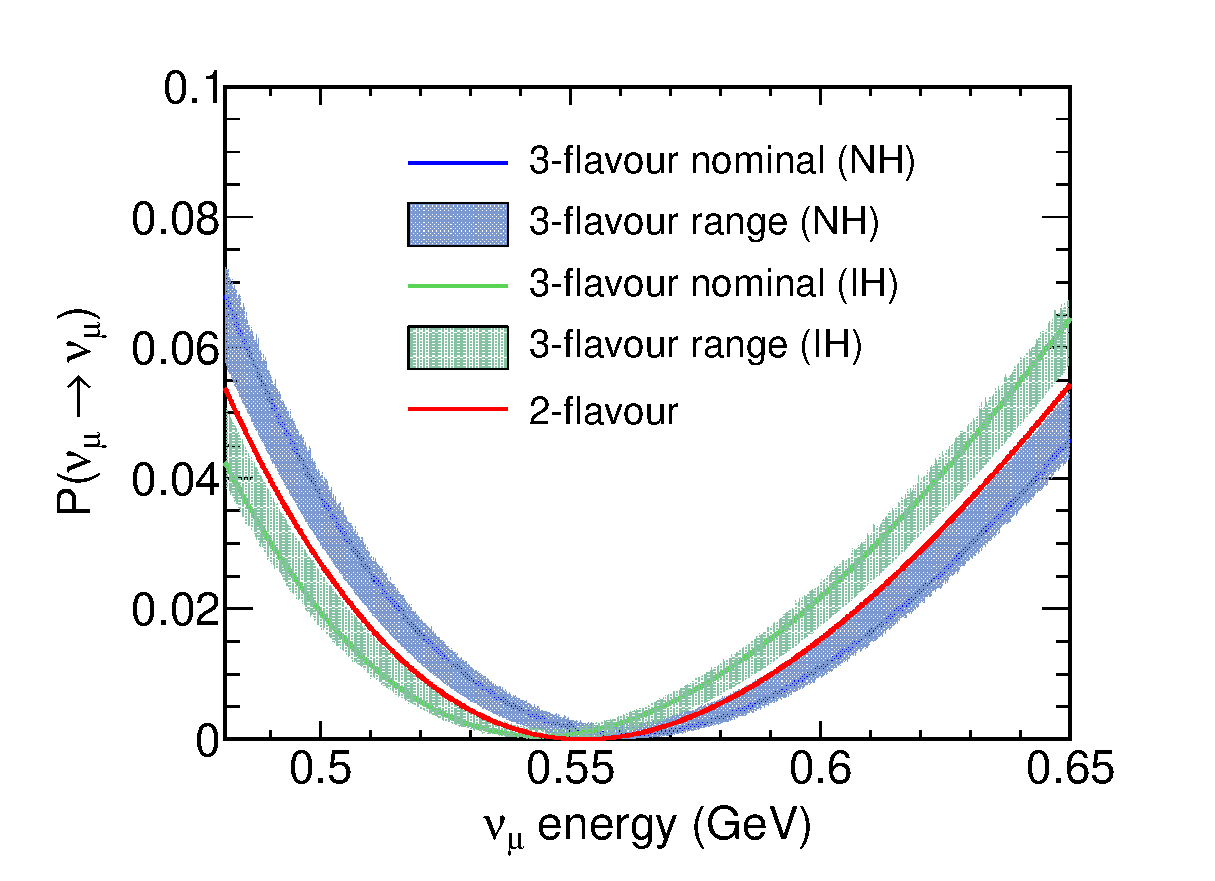
\includegraphics{./images/osc_prob/Prob3NumuSurv.eps}}
\caption[Comparison of P($\nu_{\mu} \rightarrow \nu_{\mu}$) for 2-flavour and 3-flavour (in matter) oscillations]
{Comparison of P($\nu_{\mu} \rightarrow \nu_{\mu}$) for 2-flavour and 3-flavour (in matter) oscillations, NH = normal mass hierarchy,
IH = inverted mass hierarchy. The nominal probabilities are calculated with $\sin^{2}(2 \theta_{12})$ = 0.87, $\sin^{2}(2 \theta_{13})$ = 0.1, 
$\sin^{2}(2 \theta_{23})$ = 1.0, $\Delta m_{21}^{2}$ = 7.6 $\times 10^{-5}$  eV$^{2}$/c$^{4}$, $|\Delta m_{32}^{2}|$ = 2.32 $\times$ 10$^{-3}$ eV$^{2}$/c$^{4}$, 
$\delta_{CP}$ = 0 and Earth crust density = 2.6 g/cm$^{3}$. The bands represent the maximum and minimum 3-flavour probabilities from 4000 random 
variations of the non-23 oscillation parameters within their uncertainties at each energy with the same values of $\sin^{2}(2 \theta_{23})$ and 
$|\Delta m_{32}^{2}|$ being used.}
\label{pnumunumucomp}
\end{center}
\end{figure}

\begin{figure}
\begin{center}
\resizebox{14cm}{!}{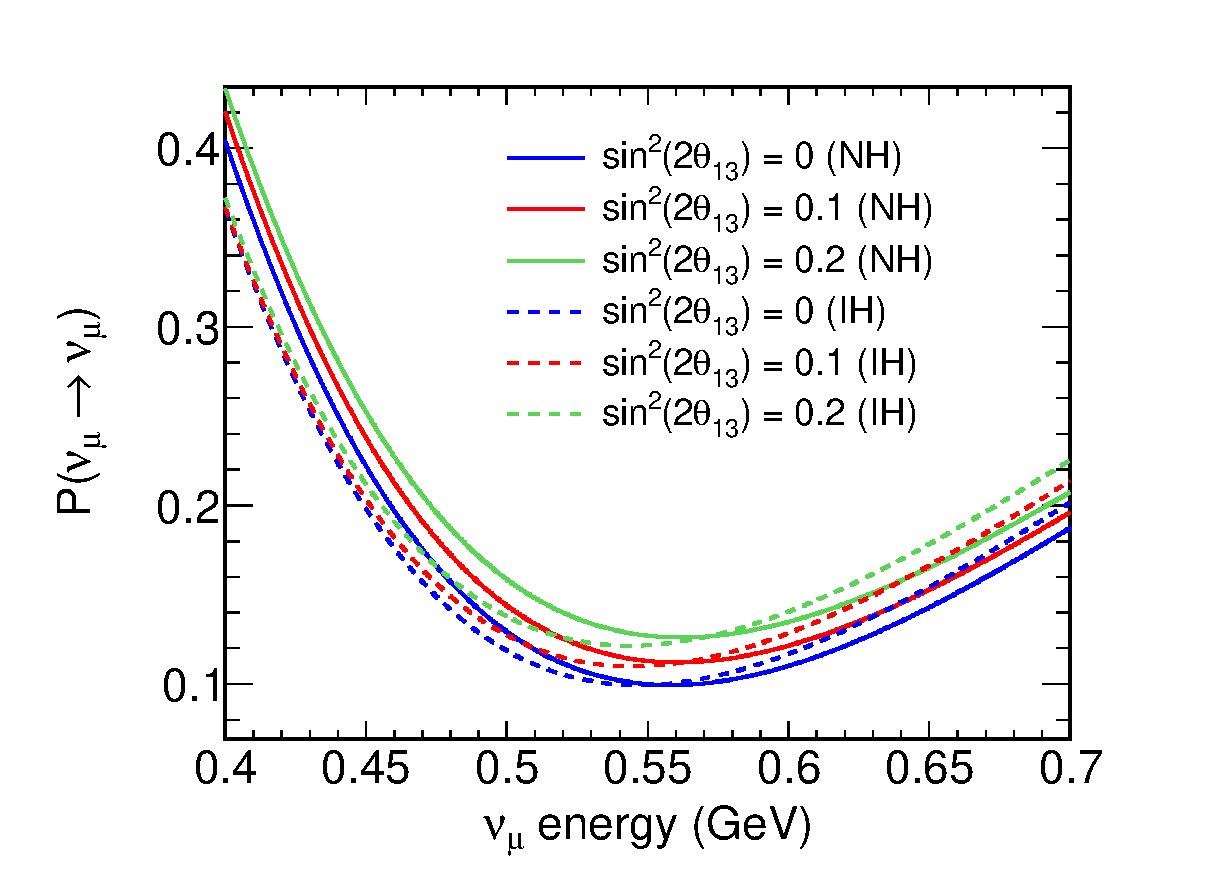
\includegraphics{./images/osc_prob/Prob3NumuSurvS13.eps}}
\caption[Effect of $\sin^{2}(2 \theta_{13})$ on P($\nu_{\mu} \rightarrow \nu_{\mu}$) for 3-flavour oscillations in matter]
{Effect of $\sin^{2}(2 \theta_{13})$ on P($\nu_{\mu} \rightarrow \nu_{\mu}$) for 3-flavour oscillations in matter; NH = 
normal mass hierarchy, IH = inverted mass hierarchy, $\sin^{2}(2 \theta_{12})$ = 0.87, $\sin^{2}(2 \theta_{23})$ = 1.0,
$\Delta m_{21}^{2}$ = 7.6 $\times 10^{-5}$ eV$^{2}$/c$^{4}$, $|\Delta m_{32}^{2}|$ = 2.32 $\times$ 10$^{-3}$ eV$^{2}$/c$^{4}$, $\delta_{CP}$ = 0
and Earth crust density = 2.6 g/cm$^{3}$}
\label{pnumunumus13}
\end{center}
\end{figure}

\begin{figure}
\begin{center}
\resizebox{14cm}{!}{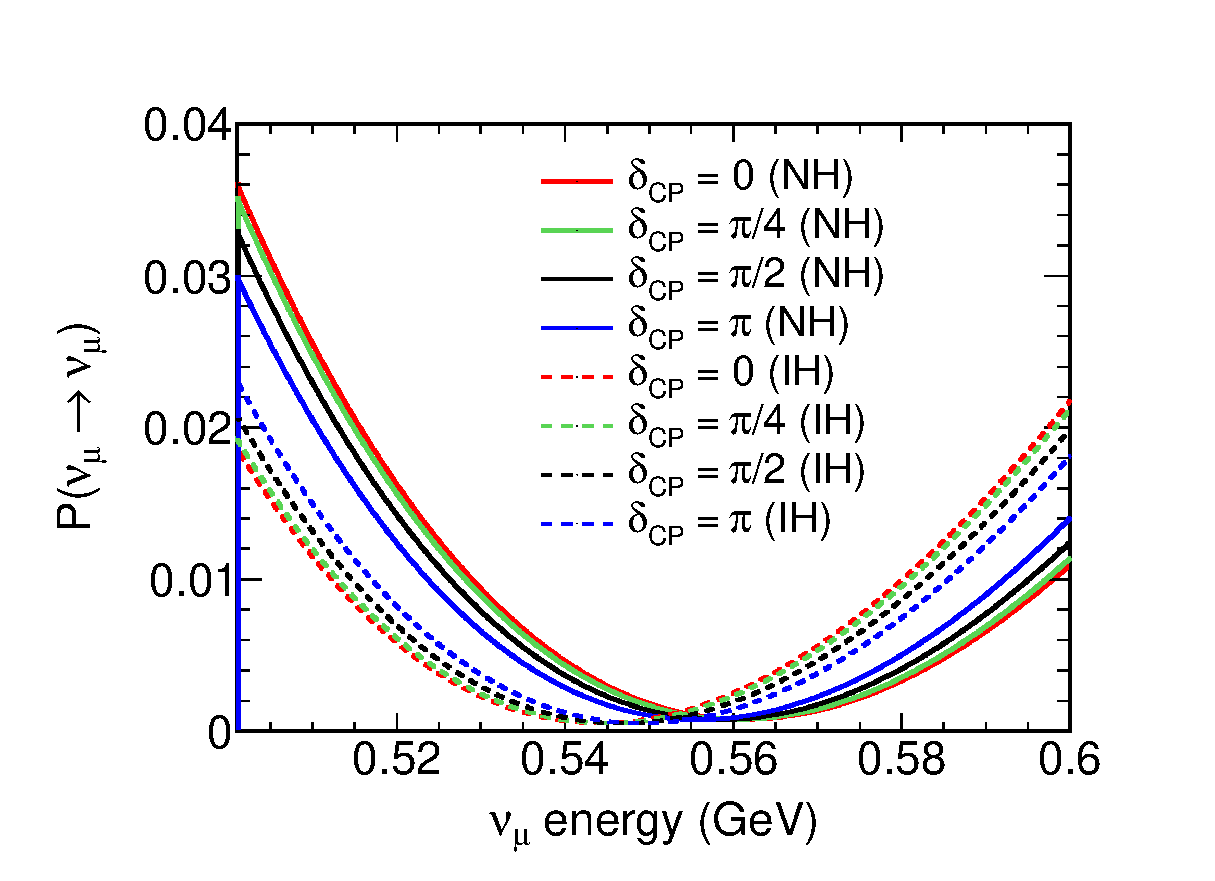
\includegraphics{./images/osc_prob/Prob3NumuSurvDeltaCP0506.eps}}
\caption[Effect of $\delta_{CP}$ on P($\nu_{\mu} \rightarrow \nu_{\mu}$) for 3-flavour oscillations in matter]
{Effect of $\delta_{CP}$ on P($\nu_{\mu} \rightarrow \nu_{\mu}$) for 3-flavour oscillations in matter; NH = normal mass hierarchy,
IH = inverted mass hierarchy, $\sin^{2}(2 \theta_{12})$ = 0.87, $\sin^{2}(2 \theta_{13})$ = 0.1, $\sin^{2}(2 \theta_{23})$ = 1.0,
$\Delta m_{21}^{2}$ = 7.6 $\times 10^{-5}$  eV$^{2}$/c$^{4}$, $|\Delta m_{32}^{2}|$ = 2.32 $\times$ 10$^{-3}$ eV$^{2}$/c$^{4}$ 
and Earth crust density = 2.6 g/cm$^{3}$}
\label{pnumunumudelta}
\end{center}
\end{figure}

%\begin{figure}
%\begin{center}
%\resizebox{14cm}{!}{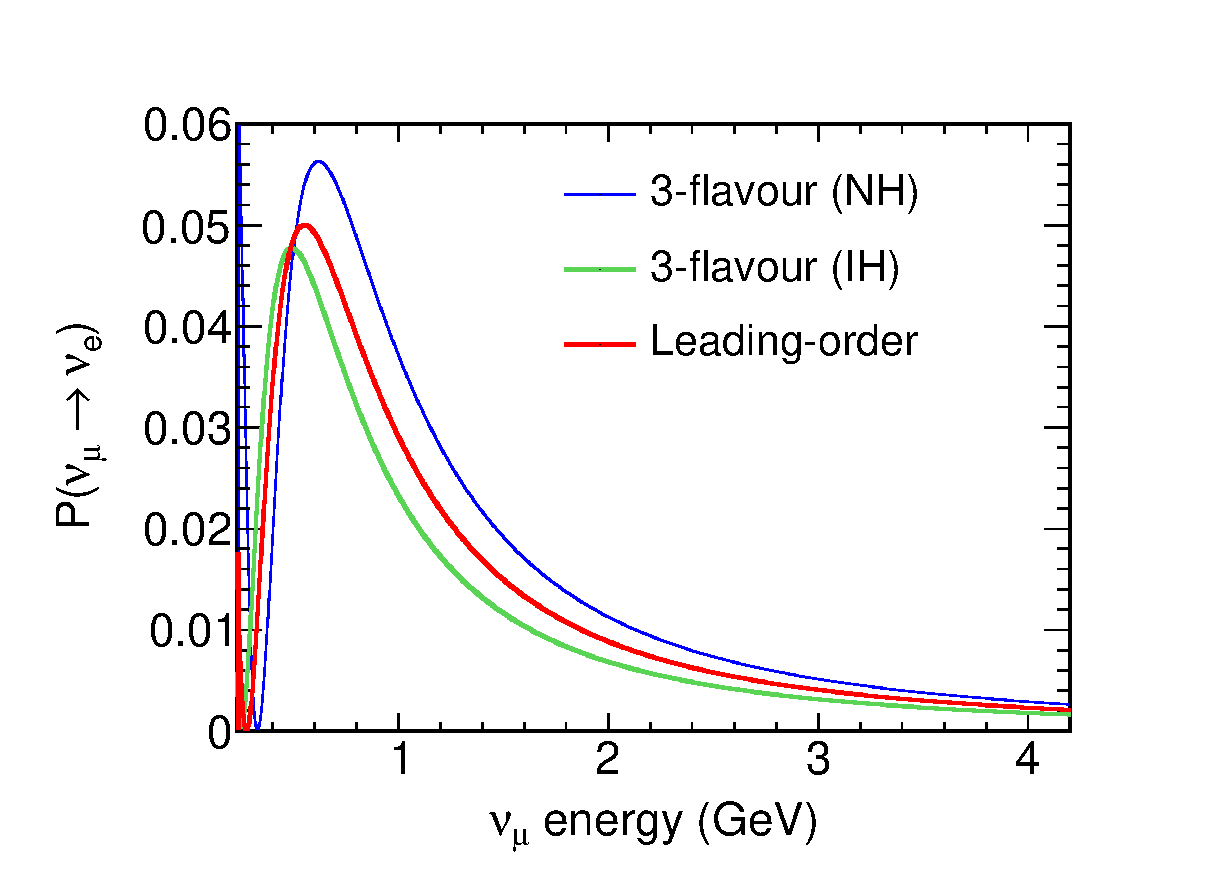
\includegraphics{./images/osc_prob/Prob3NueApp.eps}}
%\caption{Comparison of P($\nu_{\mu} \rightarrow \nu_{e}$) for leading-order and 3-flavour (in matter) oscillations; NH = normal mass hierarchy,
%IH = inverted mass hierarchy, $\sin^{2}(2 \theta_{12})$ = 0.87, $\sin^{2}(2 \theta_{13})$ = 0.1, $\sin^{2}(2 \theta_{23})$ = 1.0,
%$\Delta m_{21}^{2}$ = 7.6 $\times 10^{-5}$  eV$^{2}$/c$^{4}$, $|\Delta m_{32}^{2}|$ = 2.32 $\times$ 10$^{-3}$ eV$^{2}$/c$^{4}$, $\delta_{CP}$ = 0 
%and Earth crust density = 2.6 g/cm$^{3}$}
%\label{pnumunuecomp}
%\end{center}
%\end{figure}

%\begin{figure}
%\begin{center}
%\resizebox{14cm}{!}{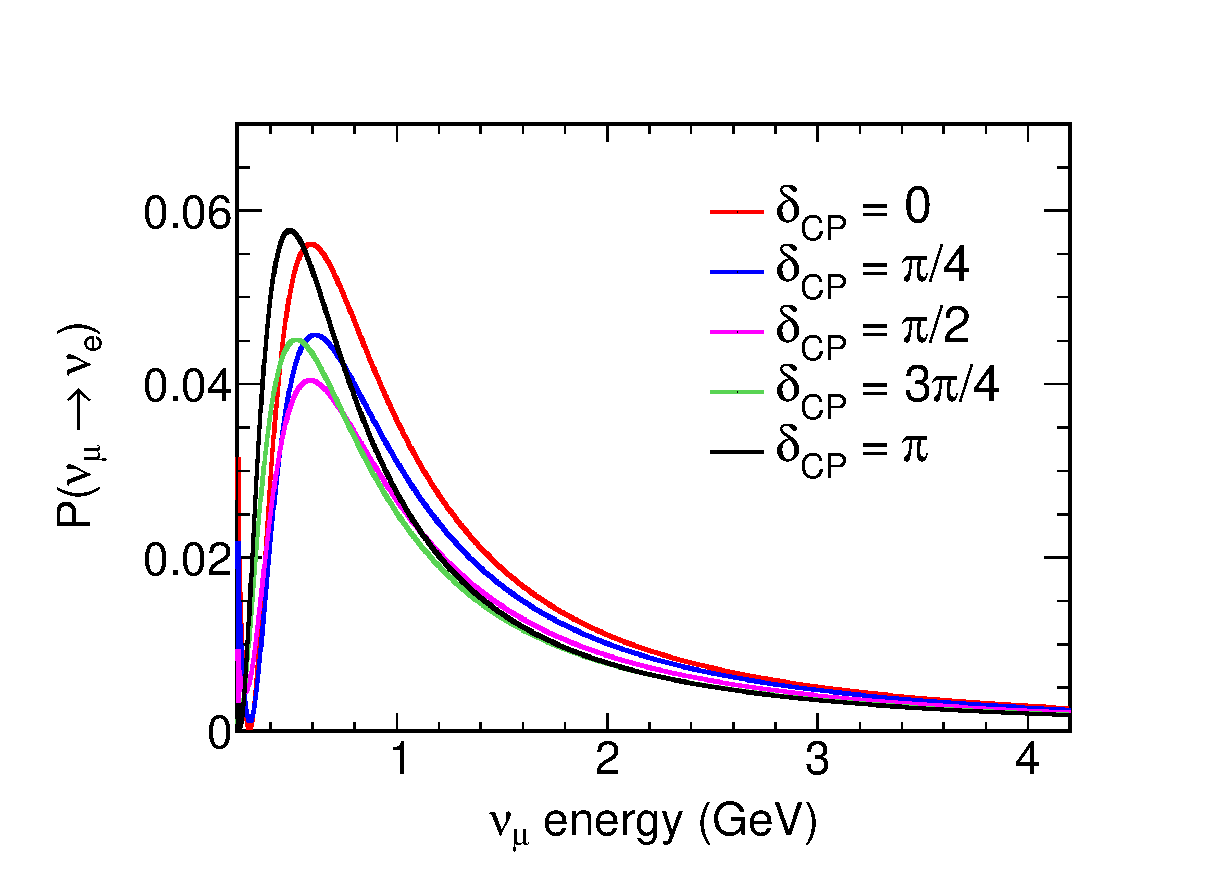
\includegraphics{./images/osc_prob/Prob3NueAppDeltaCP.eps}}
%\caption{Effect of $\delta_{CP}$ on P($\nu_{\mu} \rightarrow \nu_{e}$) for 3-flavour oscillations in matter; normal mass hierarchy,
%$\sin^{2}(2 \theta_{12})$ = 0.87, $\sin^{2}(2 \theta_{13})$ = 0.1, $\sin^{2}(2 \theta_{23})$ = 1.0,
%$\Delta m_{21}^{2}$ = 7.6 $\times 10^{-5}$  eV$^{2}$/c$^{4}$, $|\Delta m_{32}^{2}|$ = 2.32 $\times$ 10$^{-3}$ eV$^{2}$/c$^{4}$ 
%and Earth crust density = 2.6 g/cm$^{3}$}
%\label{pnumunuedelta}
%\end{center}
%\end{figure}

\begin{table}
\caption[Effects of uncertainties in $\sin^{2}(2 \theta_{12})$ and $\Delta m_{21}^{2}$ on the 3-flavour
P($\nu_{\mu} \rightarrow \nu_{\mu}$) in matter]{Effects of uncertainties in $\sin^{2}(2 \theta_{12})$ and $\Delta m_{21}^{2}$ 
on the 3-flavour P($\nu_{\mu} \rightarrow \nu_{\mu}$) in matter; this is for the normal mass hierarchy, $\sin^{2}(2 \theta_{23})$ 
= 1.0, $|\Delta m_{32}^{2}|$ = 2.32 $\times$ 10$^{-3}$ eV$^{2}$/c$^{4}$, $\sin^{2}(2 \theta_{13})$ = 0.1 and $\delta_{CP}$ = 0}
\centering
\begin{tabular}{| c | c | c | c | c | c |}
\hline
Energy & P($\nu_{\mu} \rightarrow \nu_{\mu}$) & P($\nu_{\mu} \rightarrow \nu_{\mu}$) &
       P($\nu_{\mu} \rightarrow \nu_{\mu}$) & P($\nu_{\mu} \rightarrow \nu_{\mu}$) & P($\nu_{\mu} \rightarrow \nu_{\mu}$) \\
(GeV) & for $\sin^{2}(2 \theta_{12})$ & for $\sin^{2}(2 \theta_{12})$ & for $\sin^{2}(2 \theta_{12})$
             & for $\sin^{2}(2 \theta_{12})$ & for $\sin^{2}(2 \theta_{12})$ \\
  & = 0.870, & = 0.906, & = 0.833, & = 0.870, & = 0.870, \\
  & $\Delta m_{21}^{2}$ = &  $\Delta m_{21}^{2}$ = & $\Delta m_{21}^{2}$ = & $\Delta m_{21}^{2}$ = & $\Delta m_{21}^{2}$ = \\
  & 7.6 $\times 10^{-5}$  eV$^{2}$/c$^{4}$ & 7.6 $\times 10^{-5}$  eV$^{2}$/c$^{4}$ & 7.6 $\times 10^{-5}$  eV$^{2}$/c$^{4}$ 
   & 7.8 $\times 10^{-5}$ eV$^{2}$/c$^{4}$ & 7.4 $\times 10^{-5}$  eV$^{2}$/c$^{4}$ \\
\hline
0.3 &  0.95703 &  0.95809 &  0.95608 &  0.95733 &  0.95674 \\
\hline
0.4 &  0.35053 &  0.35247 &  0.34877 &  0.35135 &  0.34971 \\
\hline
0.5 &  0.037395 &  0.038009 &  0.036842 &  0.037663 &  0.037129 \\
\hline
0.6 &  0.010963 &  0.010692 &  0.011212 &  0.010841 &  0.011086 \\
\hline
0.7 &  0.094387 &  0.093711 &  0.095004 &  0.094083 &  0.094691 \\
\hline
0.8 &  0.20453 &  0.20371 &  0.20528 &  0.20416 &  0.20490 \\
\hline
0.9 &  0.31099 &  0.31015 &  0.31175 &  0.31061 &  0.31137 \\
\hline
1.0 &  0.40463 &  0.40383 &  0.40535 &  0.40427 &  0.40499 \\
\hline
1.1 &  0.48414 &  0.48340 &  0.48481 &  0.48380 &  0.48447 \\
\hline
1.2 &  0.55080 &  0.55013 &  0.55141 &  0.55050 &  0.55111 \\
\hline
1.3 &  0.60656 &  0.60594 &  0.60711 &  0.60628 &  0.60683 \\
\hline
1.4 &  0.65329 &  0.65274 &  0.65380 &  0.65304 &  0.65354 \\
\hline
1.5 &  0.69265 &  0.69215 &  0.69311 &  0.69243 &  0.69288 \\
\hline
1.6 &  0.72599 &  0.72554 &  0.72640 &  0.72579 &  0.72620 \\
\hline
1.7 &  0.75440 &  0.75399 &  0.75478 &  0.75421 &  0.75459 \\
\hline
1.8 &  0.77876 &  0.77839 &  0.77910 &  0.77859 &  0.77893 \\
\hline
1.9 &  0.79978 &  0.79943 &  0.80009 &  0.79962 &  0.79993 \\
\hline
2.0 &  0.81801 &  0.81770 &  0.81830 &  0.81787 &  0.81815 \\
\hline
\end{tabular}
\label{numuSurvProbEffectError12}
\end{table}

\clearpage

\begin{table}
\caption[Comparison of $\nu_{\mu}$ oscillation probabilities in vacuum and matter for the normal mass hierarchy]
{Comparison of $\nu_{\mu}$ oscillation probabilities in vacuum and matter for the normal mass hierarchy, Earth crust
density = 2.6 g/cm$^{3}$, $ \sin^{2}(2 \theta_{12})$ = 0.87, $\sin^{2}(2 \theta_{13})$ = 0.1, $\sin^{2}(2 \theta_{23})$ = 1.0, 
$\Delta m_{21}^{2}$ = 7.6 $\times$ 10$^{-5}$ eV$^{2}$/c$^{4}$, $|\Delta m_{32}^{2}|$ = 2.32 $\times$ 10$^{-3}$ eV$^{2}$/c$^{4}$ and $\delta_{CP}$ = 0}
\centering
\begin{tabular}{| c | c | c | c | c | c | c |}
\hline
Energy (GeV) & \multicolumn{2}{|c|}{P($\nu_{\mu} \rightarrow \nu_{e}$)} & \multicolumn{2}{|c|}{P($\nu_{\mu} \rightarrow \nu_{\mu}$)} & \multicolumn{2}{|c|}{P($\nu_{\mu} \rightarrow \nu_{\tau}$)}\\
\hline
 & Vacuum & Matter & Vacuum & Matter & Vacuum & Matter \\
\hline
0.3 &  0.00054403 &  0.00016981 &  0.95496 &  0.95703 &  0.044501 &  0.042796\\
\hline
0.4 &  0.024253 &  0.029051 &  0.34954 &  0.35053 &  0.62621 &  0.62042\\
\hline
0.5 &  0.046291 &  0.051402 &  0.037071 &  0.037395 &  0.91664 &  0.91120\\
\hline
0.6 &  0.051975 &  0.056108 &  0.010883 &  0.010963 &  0.93714 &  0.93293\\
\hline
0.7 &  0.049739 &  0.052871 &  0.094385 &  0.094387 &  0.85588 &  0.85274\\
\hline
0.8 &  0.044830 &  0.047181 &  0.20455 &  0.20453 &  0.75062 &  0.74829\\
\hline
0.9 &  0.039478 &  0.041256 &  0.31101 &  0.31099 &  0.64951 &  0.64776\\
\hline
1.0 &  0.034502 &  0.035865 &  0.40464 &  0.40463 &  0.56085 &  0.55951\\
\hline
1.1 &  0.030139 &  0.031200 &  0.48415 &  0.48414 &  0.48571 &  0.48466\\
\hline
1.2 &  0.026403 &  0.027241 &  0.55081 &  0.55080 &  0.42279 &  0.42196\\
\hline
1.3 &  0.023233 &  0.023905 &  0.60656 &  0.60656 &  0.37021 &  0.36954\\
\hline
1.4 &  0.020548 &  0.021093 &  0.65329 &  0.65329 &  0.32616 &  0.32562\\
\hline
1.5 &  0.018268 &  0.018715 &  0.69266 &  0.69266 &  0.28908 &  0.28863\\
\hline
1.6 &  0.016325 &  0.016696 &  0.72599 &  0.72599 &  0.25769 &  0.25731\\
\hline
1.7 &  0.014661 &  0.014971 &  0.75440 &  0.75440 &  0.23094 &  0.23063\\
\hline
1.8 &  0.013228 &  0.013491 &  0.77876 &  0.77876 &  0.20801 &  0.20775\\
\hline
1.9 &  0.011988 &  0.012211 &  0.79977 &  0.79978 &  0.18824 &  0.18801\\
\hline
2.0 &  0.010908 &  0.011100 &  0.81801 &  0.81801 &  0.17108 &  0.17089\\
\hline
\end{tabular}
\label{numuOscMatterEffectsNH}
\end{table}

\begin{table}
\caption[Comparison of $\nu_{\mu}$ oscillation probabilities in vacuum and matter for the inverted mass hierarchy]
{Comparison of $\nu_{\mu}$ oscillation probabilities in vacuum and matter for the inverted mass hierarchy, Earth crust
density = 2.6 g/cm$^{3}$, $ \sin^{2}(2 \theta_{12})$ = 0.87, $\sin^{2}(2 \theta_{13})$ = 0.1, $\sin^{2}(2 \theta_{23})$ = 1.0,
$\Delta m_{21}^{2}$ = 7.6 $\times$ 10$^{-5}$ eV$^{2}$/c$^{4}$, $|\Delta m_{32}^{2}|$ = 2.32 $\times$ 10$^{-3}$ eV$^{2}$/c$^{4}$ and $\delta_{CP}$ = 0}
\centering
\begin{tabular}{| c | c | c | c | c | c | c |}
\hline
Energy (GeV) & \multicolumn{2}{|c|}{P($\nu_{\mu} \rightarrow \nu_{e}$)} & \multicolumn{2}{|c|}{P($\nu_{\mu} \rightarrow \nu_{\mu}$)} & \multicolumn{2}{|c|}{P($\nu_{\mu} \rightarrow \nu_{\tau}$)}\\
\hline
 & Vacuum & Matter & Vacuum & Matter & Vacuum & Matter \\
\hline
0.3 &  0.016651 &  0.012718 &  0.91243 &  0.91427 &  0.070915 &  0.073016\\
\hline
0.4 &  0.047961 &  0.041880 &  0.28695 &  0.28747 &  0.66509 &  0.67065\\
\hline
0.5 &   0.052910 &  0.047892 &  0.019598 &   0.019587 &  0.92749 &  0.93252\\
\hline
0.6 &  0.047803 &  0.044104 &  0.021900 &  0.021756 &  0.93030 &  0.93414\\
\hline
0.7 &  0.040787 &  0.038101 &  0.11802 &   0.11787 &  0.84120 &  0.84403\\
\hline
0.8 &  0.034297 &  0.032325 &  0.23236 &  0.23222 &  0.73335 &  0.73545\\
\hline
0.9 &  0.028857 &  0.027381 &  0.33905 &  0.33895 &  0.63210 &  0.63367\\
\hline
1.0 &  0.024433 &  0.023306 &  0.43123 &  0.43115 &  0.54434 &  0.54555\\
\hline
1.1 &  0.020858 &  0.019980 &  0.50865 &  0.50859 &  0.47049 &  0.47143\\
\hline
1.2 &  0.017960 &  0.017265 &  0.57310 &  0.57305 &  0.40894 &  0.40969\\
\hline
1.3 &  0.015595 &  0.015037 &  0.62672 &  0.62669 &  0.35768 &  0.35828\\
\hline
1.4 &  0.013649 &  0.013194 &  0.67151 &  0.67148 &  0.31485 &  0.31533\\
\hline
1.5 &  0.012034 &  0.011657 &  0.70911 &  0.70909 &  0.27886 &  0.27926\\
\hline
1.6 &  0.010681 &  0.010366 &  0.74089 &  0.74087 &  0.24843 &  0.24876\\
\hline
1.7 &  0.0095379 &  0.0092726 &  0.76792 & 0.76791 &  0.22254 &  0.22282\\
\hline
1.8 &  0.0085654 &  0.0083395 &  0.79107 &  0.79105 &  0.20037 &  0.20061\\
\hline
1.9 &   0.0077316 &  0.0075376 &  0.81101 &  0.81010 &  0.18126 &  0.18146\\
\hline
2.0 &  0.0070119 &  0.0068441 &  0.82829 &  0.82829 &  0.16470 &  0.16487\\
\hline
\end{tabular}
\label{numuOscMatterEffectsIH}
\end{table}

\clearpage

\subsection{Validation of the 3-flavour oscillation probabilities}
\label{3flavourvalidation}

The 3-flavour oscillation probabilities in vacuum were checked using an alternative formulation in equations 13.13 and 13.14 
in the PDG review \cite{pdgreview}:
\begin{equation}
P(\nu_{\alpha} \rightarrow \nu_{\beta}) = \sum_{j} |U_{\beta j}|^{2} |U_{\alpha j}|^{2} + 2 \sum_{j>k} |U_{\beta j} U_{\alpha j}^{*} U_{\alpha k} U_{\beta k}^{*}| 
\cos \left(\frac{\Delta m_{jk}^{2} L}{2E}  - \phi_{\beta \alpha;jk}  \right)
\label{3flavouroscprobvacuumpdg}
\end{equation}
where $\phi_{\beta \alpha;jk}$ = arg($U_{\beta j} U_{\alpha j}^{*} U_{\alpha k} U_{\beta k}^{*}$). $P(\bar{\nu}_{\alpha} \rightarrow \bar{\nu}_{\beta})$ 
is calculated by changing the sign of $\phi_{\beta \alpha;jk}$ in the argument of the cosine. The probabilities calculated from equation \ref{3flavouroscprobvacuumpdg} 
agreed with those calculated from equation \ref{3flavouroscprobvacuum} to 14 significant figures.

Several checks of the oscillation probabilities in constant density matter are written into the code that calculates them: 
\begin{enumerate}
\item The eigenvalues of $U M U^{\dagger}$ are checked by comparing their sum with the trace of the matrix. 
\item Each normalised eigenvector is multiplied in turn by each of the 3 matrices formed by subtracting the eigenvalues from the real parts of the 
diagonal elements of $U M U^{\dagger}$, and a check is made of the differences between these products and a zero vector. 
\item A check is made that the normalised eigenvectors of $U M U^{\dagger}$ are orthogonal by calculating the scalar product between them (the scalar product of two 
complex vectors is the product of the first vector with the complex conjugate of the second vector). 
\item A check is also made that the Hermitian conjugate of the mixing matrix in matter is equal to the inverse of the matrix. This is done by multiplying the 
mixing matrix in matter by its Hermitian conjugate, and checking the differences between the product and an identity matrix.
\end{enumerate}

The values of the oscillation probabilities in constant density matter were checked by comparing them with equivalent probabilities calculated by an 
independently-written Fortran program \cite{sloan}. This Fortran program uses different algorithms, and calculates numerically the eigenvalues and 
eigenvectors of $U M U^{\dagger}$. Nevertheless there was very good agreement between the two calculations of the probabilities, with the 
fractional differences being $\approx 2 \times 10^{-6}$. 

The values of the matter oscillation probabilities were also compared with those given by Prob3++ \cite{Prob3}, and the fractional differences were 
$\approx$ 1-5 $\times$ 10$^{-4}$. The comparison plots can be seen in \cite{Compwithprob3}.

\subsection{Accuracy of the 3-flavour oscillation probabilities} 
\label{3flavouraccuracy}

As stated in section \ref{3flavourvalidation}, the 3-flavour oscillation probabilities in vacuum agreed to 14 significant figures between the two 
formulations.

An estimate of the accuracy of the 3-flavour oscillation probabilities in constant density matter was made in three separate ways: 
\begin{enumerate}
\item The matter probabilities for zero density were compared with the vacuum probabilities; there was good agreement, with the fractional differences being 
$\approx$ 2-5 $\times$ 10$^{-6}$. 
\item The probabilites given when calculating the eigenvectors with simultaneous equations 1 and 2 in $U M U^{\dagger} - \lambda I = 0$ were compared 
with the probabilities given when calculating the eigenvectors with simultaneous equations 2 and 3. The fractional differences between these two 
calculations were again $\approx$ 2-5 $\times$ 10$^{-6}$.
\item The sum of three matter probabilities, for example P($\nu_{\mu} \rightarrow \nu_{e}$) + P($\nu_{\mu} \rightarrow \nu_{\mu}$) + 
P($\nu_{\mu} \rightarrow \nu_{\tau}$), was compared with 1.0; again there was good agreement, and the differences were $\approx 2 \times 10^{-6}$. 
\end{enumerate}

This means that the matter oscillation probabilities should be considered to be accurate to 5 decimal places. The accuracy of the matter probabilities 
is less than that of the vacuum probabilities due to the method of calculation of the eigenvectors. This involves calculations of the form 
\begin{displaymath}
\frac{(ab - cd)}{(ef - gh)}
\end{displaymath} 
where a, b, c, etc.\ are elements of $U M U^{\dagger} - \lambda I$. Frequently ab is close in value to cd, which means that (ab - cd) is much smaller than ab or 
cd, and the same applies to (ef - gh). However the advantage of the method of calculation of the eigenvectors described in section \ref{matterosc} is that it allows 
the worst of these cancellation errors to be avoided; this can be done by calculating the eigenvectors using different pairs of simultaneous equations in 
$U M U^{\dagger} - \lambda I = 0$ for different combinations of the oscillation parameters. In practice, the eigenvectors are nearly always calculated 
using equations 1 and 2 in $U M U^{\dagger} - \lambda I = 0$, but equations 2 and 3 are used when 3.10 $<$ $\delta_{CP}$ $<$ 3.18 and 
$\sin^{2}(2 \theta_{13})$ $>$ $10^{-8}$ in order to avoid such cancellation errors.  






\clearpage

\section{Updated predictions of single $\mu$-like ring spectrum in Super-K}
\label{sec:pred}

For 2-flavour oscillations, the predicted reconstructed single $\mu$-like ring spectrum in Super-K depends only on 
$\sin^{2}(2 \theta_{23})$ and $|\Delta m_{32}^{2}|$. However for the 3-flavour hypothesis, it also depends on 
$\sin^{2}(2 \theta_{13})$, $\sin^{2}(2 \theta_{12})$, $\Delta m_{21}^{2}$, $\delta_{CP}$ and the mass hierarchy. 
One other change from the 2-flavour analysis is that oscillated $\nu_{e}$ templates were added for the interaction modes CCQE, CC1$\pi$ and 
CC other. An oscillated $\nu_{e}$ template for NC was not included since the $\nu_{\mu}$ NC template effectively includes $\nu_{e}$ and 
$\nu_{\tau}$ NC.
 
The predicted numbers of events in Super-K for each interaction mode are given in table \ref{genieeventnumbers} for GENIE and in table 
\ref{neuteventnumbers} for NEUT. The 2-flavour predictions are made using $\sin^{2}(2 \theta_{23})$ = 1.0 and $|\Delta m_{32}^{2}|$ = 2.32 $\times$ 10$^{-3}$ eV$^{2}$/c$^{4}$. 
The nominal 3-flavour predictions are made with $\sin^{2}(2 \theta_{12})$ = 0.87, $\sin^{2}(2 \theta_{13})$ = 0.1, $\sin^{2}(2 \theta_{23})$ = 1.0,
$\Delta m_{21}^{2}$ = 7.6 $\times$ 10$^{-5}$ eV$^{2}$/c$^{4}$, $\delta_{CP}$ = 0 and Earth crust density = 2.6 g/cm$^{3}$; the second mass-squared difference 
is 2.32 $\times$ 10$^{-3}$ eV$^{2}$/c$^{4}$ and this is input either as $|\Delta m_{32}^{2}|$ or as $|\Delta m_{FL}^{2}|$ = $|m_{3}^{2} - [(m_{2}^{2} + m_{1}^{2}) / 2]|$. 
The ranges of 3-flavour predictions in tables \ref{genieeventnumbers} and \ref{neuteventnumbers} represent the maximum and minimum numbers from 1000 random 
variations of the non-23 parameters within their uncertainties using the same values of $\sin^{2}(2 \theta_{23})$ and the atmospheric mass-squared difference. 
When the the atmospheric $\Delta m^{2}$ is input as $|\Delta m_{32}^{2}|$, there are more $\nu_{\mu}$ CCQE and 
$\nu_{\mu}$ CC1$\pi$ events in the 3-flavour inverted-hierarchy (IH) prediction and less in the 3-flavour normal-hierarchy (NH) prediction than in the 
2-flavour prediction. This is because the $\nu_{\mu}$-survival probability is higher for the IH than the NH above the oscillation maximum and lower below 
the oscillation maximum (see figure \ref{pnumunumucomp}). Since there are more events above the oscillation maximum than below it, the total number is 
larger for the IH than for the NH. This is true for any combination of the non-23 oscillation parameters. When the the atmospheric $\Delta m^{2}$ is 
input as $|\Delta m_{FL}^{2}|$, the 3-flavour predicted numbers of events are very similar to the 2-flavour numbers; this is because $|\Delta m_{31}^{2}|$ 
is equal to $|\Delta m_{32}^{2}|$ in the 2-flavour approximation, and $|\Delta m_{FL}^{2}|$ represents the average of these two mass-squared differences.


\begin{table}
\caption[Predicted numbers of single $\mu$-like ring events in Super-K for each interaction mode using GENIE]
{Predicted numbers of single $\mu$-like ring events in Super-K for each interaction mode using GENIE. The 2-flavour predictions are made using 
$\sin^{2}(2 \theta_{23})$ = 1.0 and $|\Delta m_{32}^{2}|$ = 2.32 $\times$ 10$^{-3}$ eV$^{2}$/c$^{4}$. The nominal 3-flavour predictions are made with 
$\sin^{2}(2 \theta_{12})$ = 0.87, $\sin^{2}(2 \theta_{13})$ = 0.1, $\sin^{2}(2 \theta_{23})$ = 1.0, $\Delta m_{21}^{2}$ = 7.6 $\times$ 10$^{-5}$ eV$^{2}$/c$^{4}$, 
$\delta_{CP}$ = 0 and Earth crust density = 2.6 g/cm$^{3}$; the second mass-squared difference is 2.32 $\times$ 10$^{-3}$ eV$^{2}$/c$^{4}$ and this is input either 
as $|\Delta m_{32}^{2}|$ or as $|\Delta m_{FL}^{2}|$ = $|m_{3}^{2} - [(m_{2}^{2} + m_{1}^{2}) / 2]|$. The ranges of 3-flavour predictions represent the 
maximum and minimum numbers from 1000 random variations of the non-23 parameters within their uncertainties using the same values of $\sin^{2}(2 \theta_{23})$ 
and the atmospheric mass-squared difference. NH = normal mass hierarchy, IH = inverted mass hierarchy.}
\renewcommand{\tabcolsep}{3.5pt}
\centering
\begin{tabular}{| c | c | c | c | c | c | c | c | c | c |}
\hline
Interaction &  2-flavour & \multicolumn{2}{|c|}{3-flavour} & \multicolumn{2}{|c|}{3-flavour} & \multicolumn{2}{|c|}{3-flavour} & \multicolumn{2}{|c|}{3-flavour} \\
mode &  & \multicolumn{2}{|c|}{$|\Delta m_{32}^{2}|$} & \multicolumn{2}{|c|}{$|\Delta m_{32}^{2}|$} & \multicolumn{2}{|c|}{$|\Delta m_{FL}^{2}|$} & \multicolumn{2}{|c|}{$|\Delta m_{FL}^{2}|$} \\
 &  & \multicolumn{2}{|c|}{(matter, NH)} & \multicolumn{2}{|c|}{(matter, IH)} & \multicolumn{2}{|c|}{(matter, NH)} & \multicolumn{2}{|c|}{(matter, IH)} \\
\hline
 &   & Nominal & Range & Nominal & Range & Nominal & Range & Nominal & Range \\
\hline
Total &  28.39 & 28.14 & 28.06 & 28.87 & 28.56 & 28.51 & 28.44 & 28.45 & 28.17 \\
 &  &  & - 28.43  &  & - 28.98 &  & - 28.83 &  & - 28.52 \\
\hline
$\nu_{\mu}$ CCQE &  16.52 & 16.32 & 16.27 & 16.79 & 16.59 & 16.55 & 16.50 & 16.51 & 16.33 \\
 &  (58.1\%) & (58.0\%) & - 16.49 & (58.2\%) & - 16.87 & (58.0\%) & - 16.76 & (58.0\%) & - 16.55 \\
\hline
$\nu_{\mu}$ CC1$\pi$ &  6.68 & 6.56 & 6.55 & 6.78 & 6.70 & 6.68 & 6.66 & 6.66 & 6.58 \\
 &  (23.6\%) &(23.3\%) & - 6.64  &(23.5\%) & - 6.81 & (23.4\%) & 6.76 & (23.4\%) & - 6.68 \\
\hline
$\nu_{\mu}$ CCother &  1.11 & 1.10 & 1.10 & 1.11 & 1.11 & 1.11 & 1.11 & 1.11 & 1.10 \\
 & (3.9\%)  & (3.4\%) & - 1.10 & (3.8\%) & - 1.11 & (3.9\%) & - 1.11 & (3.9\%) & - 1.11\\
\hline
$\nu_{\mu}$ ($\nu_{\tau}$) NC &  2.12 & 2.12 & 2.12 & 2.12 & 2.12 & 2.12 & 2.12 & 2.12 & 2.12 \\
 &  (7.5\%) & (7.5\%) & - 2.12 & (7.3\%) & -2.12 & (7.4\%) & - 2.12 & (7.4\%) & - 2.12 \\
\hline
$\bar{\nu}_{\mu}$ CCQE &  1.05 & 1.05 & 1.05 & 1.07 & 1.07 & 1.07 & 1.06 & 1.06 & 1.05 \\
 &  (3.7\%) & (3.7\%) & - 1.05 & (3.7\%) & -1.08 & (3.7\%) & - 1.07 & (3.7\%) & - 1.06 \\
\hline
$\bar{\nu}_{\mu}$ CC1$\pi$ &  0.63 & 0.64 & 0.64 & 0.65 & 0.65 & 0.64 & 0.64 & 0.64 & 0.64 \\
 &  (2.3\%) & (2.3\%) & - 0.64 & (2.3\%) & - 0.65 & (2.3\%) & - 0.65 & (2.3\%) & - 0.64 \\
\hline
$\bar{\nu}_{\mu}$ CCother &  0.11 & 0.11 & 0.11 & 0.11 & 0.11 & 0.11 & 0.11 & 0.11 & 0.11 \\
 &  (0.4\%) & (0.4\%) & - 0.11 & (0.4\%) & - 0.11 & (0.4\%) & - 0.11 & (0.4\%) & - 0.11 \\
\hline
$\bar{\nu}_{\mu}$ ($\bar{\nu}_{\tau}$) NC &  0.12 & 0.12 & 0.12 & 0.12 & 0.12 & 0.12 & 0.12 & 0.12 & 0.12 \\
 &  (0.4\%) & (0.4\%) & - 0.12 & (0.4\%) & - 0.12 & (0.4\%) & - 0.12 & (0.4\%) & - 0.12 \\
\hline
$\nu_{e}$ CCQE &  0.007 & 0.006 & 0.006 & 0.007 & 0.006 & 0.006 & 0.006 & 0.007 & 0.006 \\
(background) & (0.02\%) & (0.02\%) & - 0.007 & (0.02\%) & - 0.007 & (0.02\%) & - 0.007 & (0.02\%) & - 0.007 \\
\hline
$\nu_{e}$ CC1$\pi$ &  0.004 & 0.004 & 0.004 & 0.004 & 0.004 & 0.004 & 0.004 & 0.004 & 0.004 \\
(background) & (0.01\%) & (0.01\%) & - 0.004 & (0.01\%) & - 0.004 & (0.01\%) & - 0.004 & (0.01\%) & - 0.004 \\
\hline
$\nu_{e}$ CCother &  0.001 & 0.001 & 0.001 & 0.001 & 0.001 & 0.001 & 0.001 & 0.001 & 0.001 \\
(background) & (0.003\%) & (0.003\%) & - 0.001 & (0.003\%) & - 0.001 & (0.003\%) & - 0.001 & (0.003\%) & - 0.001 \\
\hline
$\nu_{e}$ NC & 0.06 & 0.06 & 0.06 & 0.06 & 0.06 & 0.06 & 0.06 & 0.06 & 0.06 \\
(background) & (0.2\%) & (0.2\%) & - 0.06  & (0.2\%) & - 0.06 & (0.2\%) & - 0.06 & (0.2\%) & - 0.06 \\
\hline
$\nu_{e}$ CCQE &  & 0.04 & 0.02 & 0.04 & 0.02  & 0.04 & 0.02 & 0.04 & 0.01 \\
(oscillated) &  & (0.1\%) & - 0.07 & (0.1\%) & - 0.06 & (0.1\%) & - 0.07 & (0.1\%) & - 0.06 \\
\hline
$\nu_{e}$ CC1$\pi$ &  & 0.01 & 0.004 & 0.01 & 0.004 & 0.01 & 0.005 & 0.01 & 0.005 \\
(oscillated) &  & (0.04\%) & - 0.02 & (0.03\%)  & - 0.017 & (0.05\%) & - 0.02 & (0.04\%) & - 0.017 \\
\hline
$\nu_{e}$ CCother &  & 0.0006 & 0.0002 & 0.0004 & 0.0002 & 0.0006 & 0.0002 & 0.0004 & 0.0002 \\
(oscillated) &  & (0.002\%) & - 0.0008 & (0.001\%) & - 0.0007 & (0.002\%) & - 0.0009 & (0.001\%) & - 0.0007 \\
\hline
\end{tabular}
\label{genieeventnumbers}
\end{table}

\begin{table}
\caption[Predicted numbers of single $\mu$-like ring events in Super-K for each interaction mode using NEUT]
{Predicted numbers of single $\mu$-like ring events in Super-K for each interaction mode using NEUT. The 2-flavour predictions are made using
$\sin^{2}(2 \theta_{23})$ = 1.0 and $|\Delta m_{32}^{2}|$ = 2.32 $\times$ 10$^{-3}$ eV$^{2}$/c$^{4}$. The nominal 3-flavour predictions are made with
$\sin^{2}(2 \theta_{12})$ = 0.87, $\sin^{2}(2 \theta_{13})$ = 0.1, $\sin^{2}(2 \theta_{23})$ = 1.0, $\Delta m_{21}^{2}$ = 7.6 $\times$ 10$^{-5}$ eV$^{2}$/c$^{4}$,
$\delta_{CP}$ = 0 and Earth crust density = 2.6 g/cm$^{3}$; the second mass-squared difference is 2.32 $\times$ 10$^{-3}$ eV$^{2}$/c$^{4}$ and this is input either
as $|\Delta m_{32}^{2}|$ or as $|\Delta m_{FL}^{2}|$ = $|m_{3}^{2} - [(m_{2}^{2} + m_{1}^{2}) / 2]|$. The ranges of 3-flavour predictions represent the
maximum and minimum numbers from 1000 random variations of the non-23 parameters within their uncertainties using the same values of $\sin^{2}(2 \theta_{23})$
and the atmospheric mass-squared difference. NH = normal mass hierarchy, IH = inverted mass hierarchy.}
\renewcommand{\tabcolsep}{3.5pt}
\centering
\begin{tabular}{| c | c | c | c | c | c | c | c | c | c |}
\hline
Interaction &  2-flavour & \multicolumn{2}{|c|}{3-flavour} & \multicolumn{2}{|c|}{3-flavour} & \multicolumn{2}{|c|}{3-flavour} & \multicolumn{2}{|c|}{3-flavour} \\
mode &  & \multicolumn{2}{|c|}{$|\Delta m_{32}^{2}|$} & \multicolumn{2}{|c|}{$|\Delta m_{32}^{2}|$} & \multicolumn{2}{|c|}{$|\Delta m_{FL}^{2}|$} & \multicolumn{2}{|c|}{$|\Delta m_{FL}^{2}|$} \\
 &  & \multicolumn{2}{|c|}{(matter, NH)} & \multicolumn{2}{|c|}{(matter, IH)} & \multicolumn{2}{|c|}{(matter, NH)} & \multicolumn{2}{|c|}{(matter, IH)} \\
\hline
 &   & Nominal & Range & Nominal & Range & Nominal & Range & Nominal & Range \\
\hline
Total & 29.18 & 28.86  & 28.79 &  29.74 & 29.40 & 29.31 & 29.23 & 29.23 & 28.92 \\
 &  &   & - 29.26  &   & - 29.86 & & - 29.70 &  & - 29.33 \\
\hline
$\nu_{\mu}$ CCQE & 16.73 & 16.49 & 16.45 & 17.08 & 16.85 & 16.79 & 16.73 & 16.74 & 16.54 \\
 &(57.3\%) &  (57.1\%) & - 16.75 & (57.5\%) & - 17.17 & (57.3\%) & - 17.05 & (57.3\%) & - 16.80 \\
\hline
$\nu_{\mu}$ CC1$\pi$ & 7.01 &  6.90 & 6.87 & 7.14 & 7.05 & 7.02 & 7.00 & 7.01 & 6.93 \\
 & (24.0\%) & (23.9\%) & - 6.99 & (24.0\%) & - 7.16 & (24.0\%) & - 7.11 & (24.0\%) & - 7.03 \\
\hline
$\nu_{\mu}$ CCother & 1.80 & 1.79  & 1.79 &  1.81 & 1.80 & 1.80 & 1.80 & 1.80 & 1.79 \\
 & (6.2\%) & (6.2\%)  & - 1.80 &  (6.1\%) & - 1.81 &  (6.1\%) & - 1.81 &  (6.2\%) & - 1.80 \\
\hline
$\nu_{\mu}$ ($\nu_{\tau}$) NC & 1.68 & 1.69 & 1.69 & 1.69 & 1.69 & 1.69 & 1.69 & 1.69 & 1.69 \\
 & (5.7\%) & (5.8\%) & - 1.69 &  (5.7\%) & - 1.69 &  (5.8\%) & - 1.69 &  (5.8\%) & - 1.69 \\
\hline
$\bar{\nu}_{\mu}$ CCQE & 1.11 &  1.10 & 1.10 &  1.13 & 1.12 & 1.11 & 1.11 & 1.11 & 1.10 \\
 & (3.8\%) &  (3.8\%) & - 1.11 &  (3.8\%) & - 1.13 &  (3.8\%) & - 1.12 &  (3.8\%) & - 1.11 \\
\hline
$\bar{\nu}_{\mu}$ CC1$\pi$ & 0.51 &  0.51 & 0.50 &  0.51 & 0.51 & 0.51 & 0.51 & 0.51 & 0.51 \\
 & (1.7\%) &  (1.8\%) & - 0.51 &  (1.7\%) & - 0.52 &  (1.7\%) & - 0.51 &  (1.7\%) & 0.51 \\
\hline
$\bar{\nu}_{\mu}$ CCother & 0.17 &  0.17 & 0.17 & 0.17 & 0.17 & 0.17 & 0.17 & 0.17 & 0.17 \\
 & (0.6\%) &  (0.6\%) & - 0.17 &  (0.6\%) & - 0.17 &  (0.6\%) & - 0.17 &  (0.6\%) & - 0.17 \\
\hline
$\bar{\nu}_{\mu}$ ($\bar{\nu}_{\tau}$) NC & 0.093 & 0.093 & 0.093 &  0.093 & 0.093 & 0.093 & 0.093 & 0.093 & 0.093 \\
 & (0.3\%) & (0.3\%) & - 0.093 &  (0.3\%) & - 0.093 &  (0.3\%) & - 0.093 &  (0.3\%) & 0.093 \\
\hline
$\nu_{e}$ CCQE & 0.008 &  0.007 & 0.007 & 0.007 & 0.007 & 0.007 & 0.007 & 0.007 & 0.007 \\
(background) & (0.03\%) &  (0.02\%) & - 0.007 & (0.02\%) & - 0.007 &  (0.02\%) & - 0.007 &  (0.02\%) & - 0.007 \\
\hline
$\nu_{e}$ CC1$\pi$ & 0.005 & 0.004 & 0.004 &  0.004 & 0.004 & 0.004 & 0.004 & 0.004 & 0.004 \\
(background) & (0.02\%) & (0.02\%) & - 0.004 & (0.01\%) & - 0.004 & (0.01\%)  & 0.004 & (0.01\%) & - 0.004 \\
\hline
$\nu_{e}$ CCother & 0.002 &  0.001 & 0.001 & 0.001 & 0.001 & 0.001 & 0.001 & 0.001 & 0.001 \\
(background) & (0.006\%) &  (0.005\%) & - 0.001 &  (0.005\%) & - 0.001 &  (0.005\%) & - 0.001 &  (0.005\%) & - 0.001 \\
\hline
$\nu_{e}$ NC & 0.05 &  0.05 & 0.05 & 0.05 & 0.05 & 0.05 & 0.05 & 0.05 & 0.05 \\
(background) & (0.2\%) &  (0.2\%) & - 0.05 &  (0.2\%) & - 0.05 &  (0.2\%) & - 0.05 &  (0.2\%) & - 0.05 \\
\hline
$\nu_{e}$ CCQE &  &  0.04 & 0.02 & 0.04 & 0.02 & 0.04 & 0.02 & 0.04 & 0.02 \\
(oscillated) &  &  (0.1\%) & - 0.07 & (0.1\%) & - 0.06 & (0.1\%) & - 0.07 & (0.1\%) & - 0.06 \\
\hline
$\nu_{e}$ CC1$\pi$ &   &  0.015 & 0.006 & 0.01 & 0.006& 0.01 & 0.005 & 0.01 & 0.005 \\
(oscillated) &  &  (0.04\%) & - 0.023 & (0.04\%) & - 0.020 & (0.05\%) & - 0.022 & (0.04\%) & - 0.021 \\
\hline
$\nu_{e}$ CCother &  &  0.001 & 0.0007 &  0.001 & 0.0006 & 0.001 & 0.0005 & 0.001 & 0.0005 \\
(oscillated) &  &  (0.005\%) & - 0.0022 &  (0.004\%) & - 0.0019 &  (0.005\%) & - 0.0021 &  (0.004\%) & - 0.0020\\
\hline
\end{tabular}
\label{neuteventnumbers}
\end{table}


The predicted reconstructed single-ring $\mu$-like Super-K spectrum using GENIE is shown in the upper plot of figure \ref{sknominalgenie}. In this plot, 
3-flavour spectra are shown both for the value 2.32 $\times$ 10$^{-3}$ eV$^{2}$/c$^{4}$ input as $|\Delta m_{32}^{2}|$ and for the same value input as 
$|\Delta m_{FL}^{2}|$ for both the NH and IH. The 2-flavour predicted spectrum is also shown for comparison. The lower plot shows the ratios of all four 
3-flavour spectra to the 2-flavour spectrum. The equivalent plots using NEUT are shown in figure \ref{sknominalneut}. These figures also show that, when 
the atmospheric $\Delta m^{2}$ is input as $|\Delta m_{32}^{2}|$, more events are predicted above the oscillation maximum and less below it for the IH 
than for the NH. When the the atmospheric $\Delta m^{2}$ is input as $|\Delta m_{FL}^{2}|$, they show that the 3-flavour predicted spectra are very similar 
to the 2-flavour spectra.

The effects of uncertainties in the non-23 oscillation parameters on the predicted reconstructed single-ring $\mu$-like Super-K spectrum are 
shown in figures \ref{skratiotheta13}, \ref{skratiodeltacp}, \ref{skratiotheta12} and \ref{skratiodm12sq}. For greater clarity, these effects are shown 
as ratios of the spectrum for $\pm$1$\sigma$ variations of a single oscillation parameter to that for the nominal value of that parameter, with the 
other five oscillation parameters being fixed. The uncertainties in $\sin^{2}(2 \theta_{12})$ and $\Delta m_{21}^{2}$ are taken from KamLAND combined 
with solar experiments \cite{Kamland}, while those in $\sin^{2}(2 \theta_{13})$ are computed as a weighted average of measurements from Daya Bay 
\cite{DayaBay} and Reno \cite{Reno}. 

By far the largest effect on the Super-K spectrum is from uncertainties in $\delta_{CP}$: changing this parameter from 0 to $\pi$ results in an 
increase of up to 5\% in the spectrum above the oscillation maximum and a decrease of up to 3\% below it for the NH. These changes 
in the spectrum are due to the changes in P($\nu_{\mu}\rightarrow\nu_{\mu}$) for different values of $\delta_{CP}$ shown in figure \ref{pnumunumudelta} 
and described in section \ref{sec:nuosc3f}. The effect 
of $\delta_{CP}$ on the predicted Super-K spectrum depends on the value of $\theta_{13}$ since the $e^{i\delta}$ terms in the PMNS matrix 
(equation \ref{PMNSmatrix}) are always multiplied by $\sin(\theta_{13})$; in figure \ref{skratiodeltacp}, $\sin^{2}(2 \theta_{13})$ has the value 
0.1. The effects of uncertainties in the other three non-23 parameters are smaller, and in all cases change the predicted Super-K spectrum by 
$\leq$ 0.5\%. For the NH, an increase in the values of both $\sin^{2}(2 \theta_{12})$ and $\Delta m_{21}^{2}$ results in an increase 
in the predicted numbers of events at energies below the oscillation maximum, and a decrease in them above the oscillation maximum; these changes 
are due to the changes in P($\nu_{\mu}\rightarrow\nu_{\mu}$) for different values of $\sin^{2}(2 \theta_{12})$ and $\Delta m_{21}^{2}$ shown in 
table \ref{numuSurvProbEffectError12}. The effects of 
$\delta_{CP}$, $\sin^{2}(2 \theta_{12})$ and $\Delta m_{21}^{2}$ are all reversed for the inverted hierarchy. The effect of an increase in 
$\sin^{2}(2 \theta_{13})$ is to increase the predicted number of events in Super-K for both hierarchies, while a decrease in this parameter results 
in a decrease in the predicted number. This is because an increase in $\sin^{2}(2 \theta_{13})$ increases P($\nu_{\mu}\rightarrow\nu_{\mu}$) for a 
given value of $\sin^{2}(2 \theta_{23})$ as shown in figure \ref{pnumunumus13}, i.e.\ more $\nu_{\mu}$ survive for higher values of $\sin^{2}(2 \theta_{13})$.

\begin{figure}
\begin{center}
\resizebox{14cm}{!}{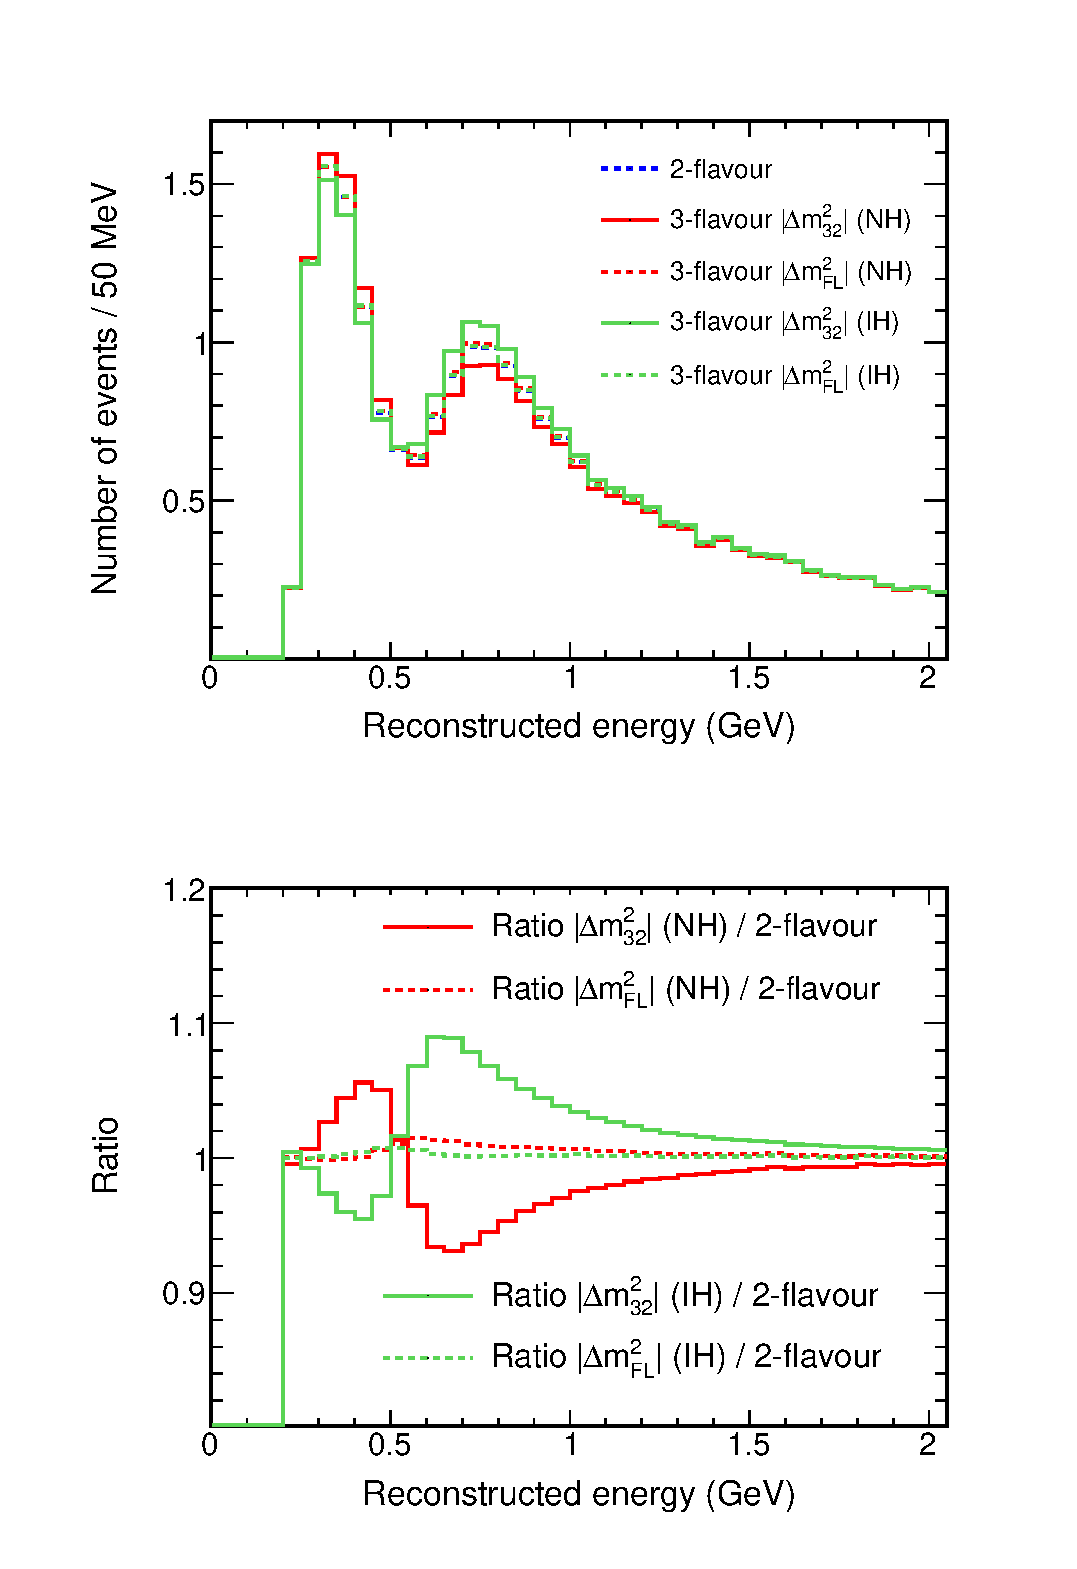
\includegraphics{./images/predicted_spectrum/SKErecoNominalGenie.eps}}
\caption[Predicted reconstructed single $\mu$-like ring spectra in Super-K for the 2-flavour and 3-flavour (in matter) hypotheses using GENIE (top plot) 
and ratios of the 3-flavour spectra to the 2-flavour spectrum (bottom plot)]
{Predicted reconstructed single $\mu$-like ring spectra in Super-K for the 2-flavour and 3-flavour (in matter) hypotheses using GENIE (top); for the 
3-flavour spectra, the value 2.32 $\times$ 10$^{-3}$ eV$^{2}$/c$^{4}$ input either as $|\Delta m_{32}^{2}|$ or as $|\Delta m_{FL}^{2}|$
= $|m_{3}^{2} - [(m_{2}^{2} + m_{1}^{2}) / 2]|$. The ratios of the 3-flavour spectra to the 2-flavour spectrum are shown in the bottom plot;  
$\sin^{2}(2 \theta_{12})$ = 0.87, $\sin^{2}(2 \theta_{13})$ = 0.1, $\sin^{2}(2 \theta_{23})$ = 1.0, $\Delta m_{21}^{2}$ = 7.6 $\times 10^{-5}$ eV$^{2}$/c$^{4}$, 
$\delta_{CP}$ = 0, Earth crust density = 2.6 g/cm$^{3}$, NH = normal mass hierarchy and IH = inverted mass hierarchy.}
\label{sknominalgenie}
\end{center}
\end{figure}

\begin{figure}
\begin{center}
\resizebox{14cm}{!}{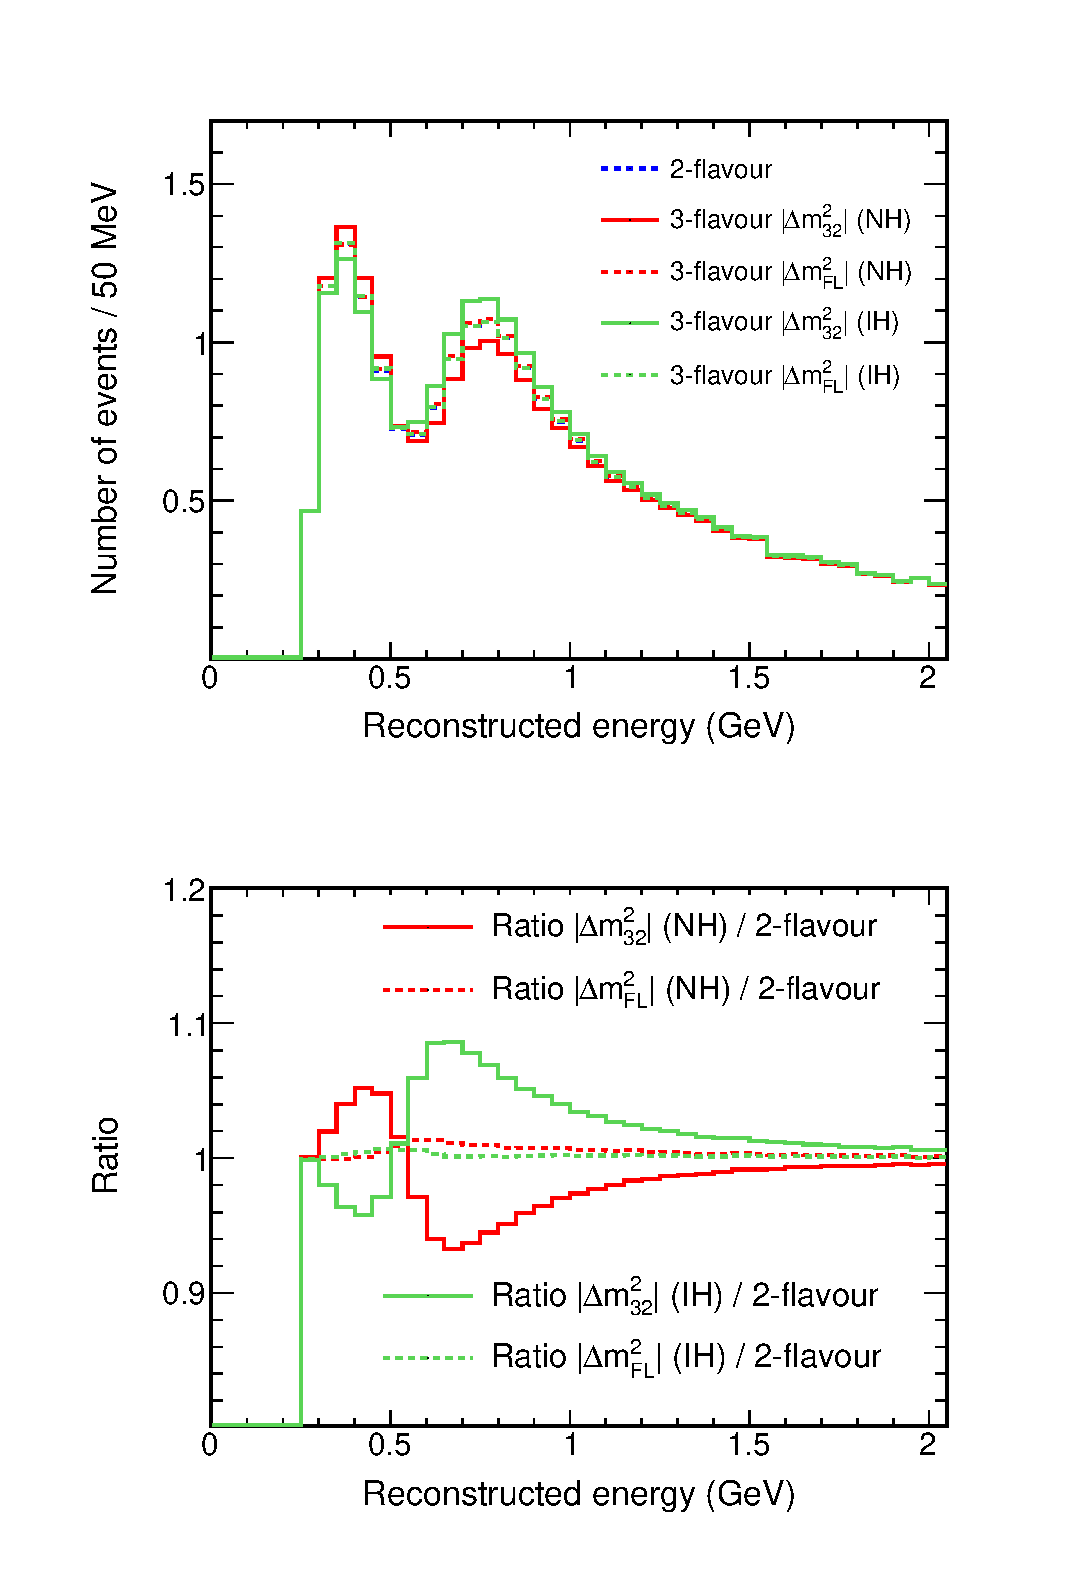
\includegraphics{./images/predicted_spectrum/SKErecoNominalNeut.eps}}
\caption[Predicted reconstructed single $\mu$-like ring spectra in Super-K for the 2-flavour and 3-flavour (in matter) hypotheses using NEUT (top plot)
and ratios of the 3-flavour spectra to the 2-flavour spectrum (bottom plot)]
{Predicted reconstructed single $\mu$-like ring spectra in Super-K for the 2-flavour and 3-flavour (in matter) hypotheses using NEUT (top); for the 
3-flavour spectra, the value 2.32 $\times$ 10$^{-3}$ eV$^{2}$/c$^{4}$ input either as $|\Delta m_{32}^{2}|$ or as $|\Delta m_{FL}^{2}|$
= $|m_{3}^{2} - [(m_{2}^{2} + m_{1}^{2}) / 2]|$. The ratios of the 3-flavour spectra to the 2-flavour spectrum are shown in the bottom plot;
$\sin^{2}(2 \theta_{12})$ = 0.87, $\sin^{2}(2 \theta_{13})$ = 0.1, $\sin^{2}(2 \theta_{23})$ = 1.0, $\Delta m_{21}^{2}$ = 7.6 $\times 10^{-5}$ eV$^{2}$/c$^{4}$,
$\delta_{CP}$ = 0, Earth crust density = 2.6 g/cm$^{3}$, NH = normal mass hierarchy and IH = inverted mass hierarchy.}
\label{sknominalneut}
\end{center}
\end{figure}

\clearpage

\begin{figure}
\begin{center}
\resizebox{13cm}{!}{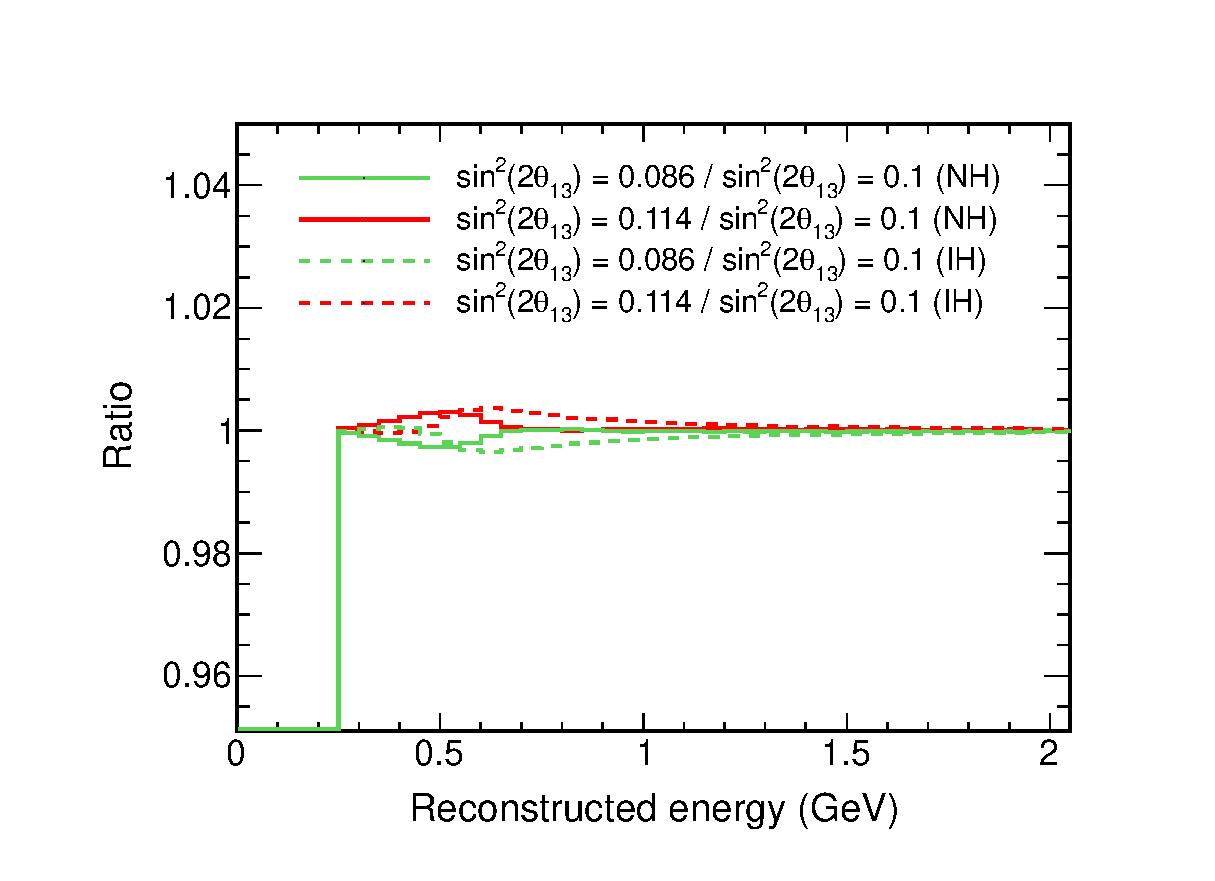
\includegraphics{./images/predicted_spectrum/SKErecoRatioTheta13.eps}}
\caption[Ratios of predicted reconstructed single $\mu$-like ring spectra in Super-K for $\pm$1$\sigma$ variations in
$\sin^{2}(2 \theta_{13})$ to those for the nominal value using NEUT]
{Ratios of predicted reconstructed single $\mu$-like ring spectra in Super-K for $\pm$1$\sigma$ variations in 
$\sin^{2}(2 \theta_{13})$ to those for the nominal value using NEUT; $\sin^{2}(2 \theta_{12})$ = 0.87, $\sin^{2}(2 \theta_{23})$ = 1.0, 
$\Delta m_{21}^{2}$ = 7.6 $\times 10^{-5}$ eV$^{2}$/c$^{4}$, $|\Delta m_{32}^{2}|$ = 2.32 $\times$ 10$^{-3}$ eV$^{2}$/c$^{4}$, $\delta_{CP}$ = 0, 
Earth crust density = 2.6 g/cm$^{3}$, NH = normal mass hierarchy and IH = inverted mass hierarchy}
\label{skratiotheta13}
\end{center}
\end{figure}

\begin{figure}
\begin{center}
\resizebox{13cm}{!}{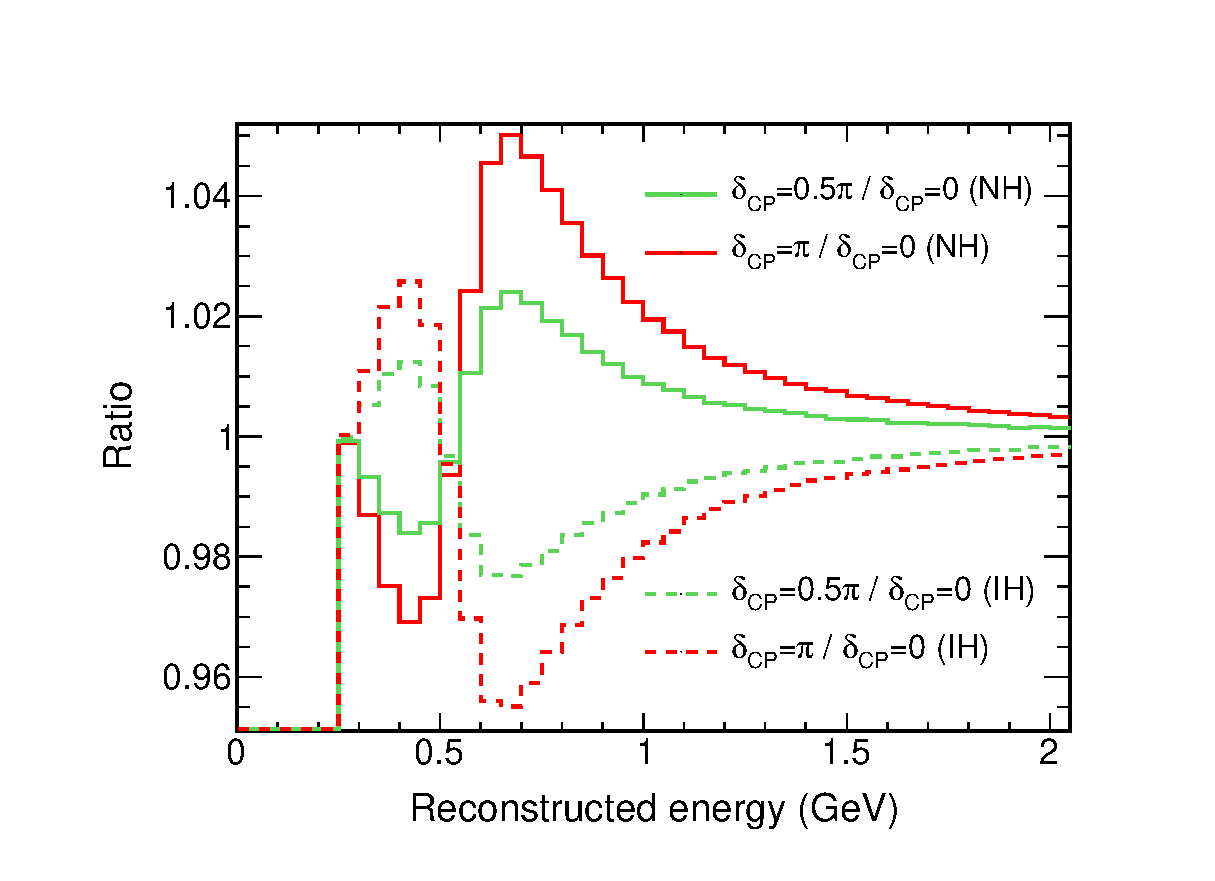
\includegraphics{./images/predicted_spectrum/SKErecoRatioDeltaCP.eps}}
\caption[Ratios of predicted reconstructed single $\mu$-like ring spectra in Super-K for $\delta_{CP}$ = $\pi$/2 and
$\delta_{CP}$ = $\pi$ to those for $\delta_{CP}$ = 0 using NEUT]
{Ratios of predicted reconstructed single $\mu$-like ring spectra in Super-K for $\delta_{CP}$ = $\pi$/2 and 
$\delta_{CP}$ = $\pi$ to those for $\delta_{CP}$ = 0 using NEUT; $\sin^{2}(2 \theta_{12})$ = 0.87, $\sin^{2}(2 \theta_{13})$ = 0.1, 
$\sin^{2}(2 \theta_{23})$ = 1.0, $\Delta m_{21}^{2}$ = 7.6 $\times 10^{-5}$ eV$^{2}$/c$^{4}$,$|\Delta m_{32}^{2}|$ 
= 2.32 $\times$ 10$^{-3}$ eV$^{2}$/c$^{4}$, Earth crust density = 2.6 g/cm$^{3}$, NH = normal mass hierarchy and IH = inverted mass hierarchy}
\label{skratiodeltacp}
\end{center}
\end{figure}

\clearpage

\begin{figure}
\begin{center}
\resizebox{13cm}{!}{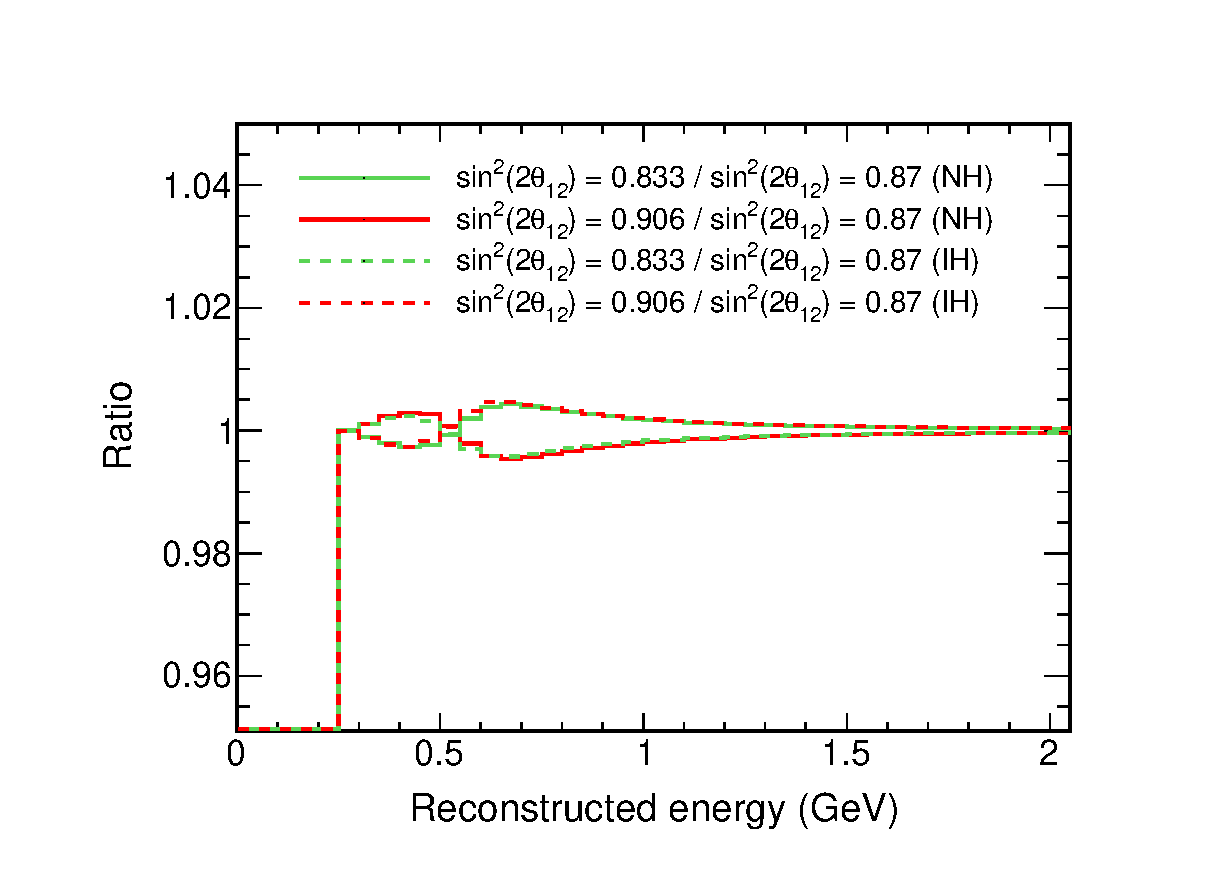
\includegraphics{./images/predicted_spectrum/SKErecoRatioTheta12.eps}}
\caption[Ratios of predicted reconstructed single $\mu$-like ring spectra in Super-K for $\pm$1$\sigma$ variations in
$\sin^{2}(2 \theta_{12})$ to those for the nominal value using NEUT]
{Ratios of predicted reconstructed single $\mu$-like ring spectra in Super-K for $\pm$1$\sigma$ variations in
$\sin^{2}(2 \theta_{12})$ to those for the nominal value using NEUT; $\sin^{2}(2 \theta_{13})$ = 0.1, $\sin^{2}(2 \theta_{23})$ = 1.0,
$\Delta m_{21}^{2}$ = 7.6 $\times 10^{-5}$ eV$^{2}$/c$^{4}$, $|\Delta m_{32}^{2}|$ = 2.32 $\times$ 10$^{-3}$ eV$^{2}$/c$^{4}$, $\delta_{CP}$ = 0, 
Earth crust density = 2.6 g/cm$^{3}$, NH = normal mass hierarchy and IH = inverted mass hierarchy}
\label{skratiotheta12}
\end{center}
\end{figure}

\begin{figure}
\begin{center}
\resizebox{13cm}{!}{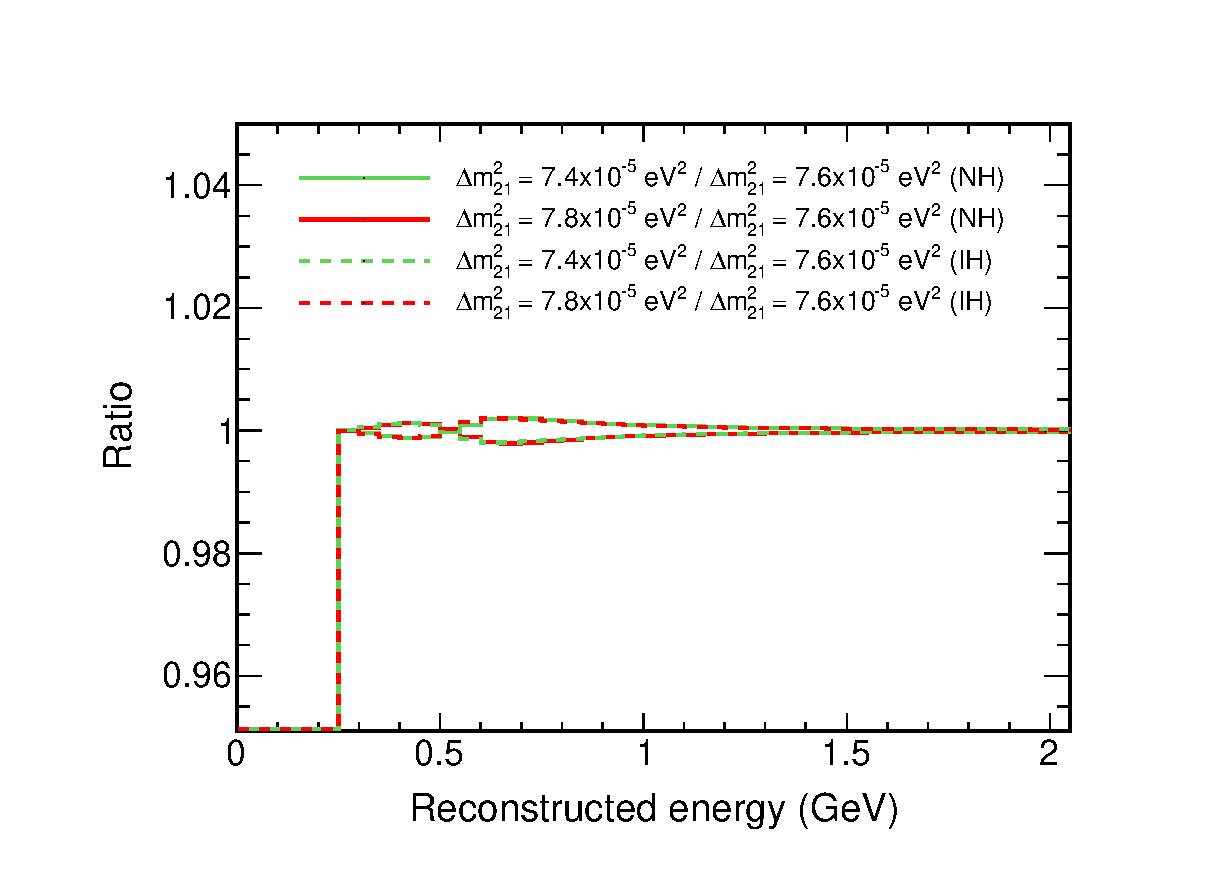
\includegraphics{./images/predicted_spectrum/SKErecoRatioDm12sq.eps}}
\caption[Ratios of predicted reconstructed single $\mu$-like ring spectra in Super-K for $\pm$1$\sigma$ variations in
$\Delta m_{21}^{2}$ to those for the nominal value using NEUT]
{Ratios of predicted reconstructed single $\mu$-like ring spectra in Super-K for $\pm$1$\sigma$ variations in
$\Delta m_{21}^{2}$ to those for the nominal value using NEUT; $\sin^{2}(2 \theta_{12})$ = 0.87, $\sin^{2}(2 \theta_{13})$ = 0.1, 
$\sin^{2}(2 \theta_{23})$ = 1.0, $|\Delta m_{32}^{2}|$ = 2.32 $\times$ 10$^{-3}$ eV$^{2}$/c$^{4}$, $\delta_{CP}$ = 0, Earth 
crust density = 2.6 g/cm$^{3}$, NH = normal mass hierarchy and IH = inverted mass hierarchy}
\label{skratiodm12sq}
\end{center}
\end{figure}

\clearpage












\clearpage

\section{3-flavour $\nu_{\mu}$-disappearance fits to the Run 1+2 dataset}
\label{sec:fits}

The best-fit values of $\sin^{2}(2 \theta_{23})$ and $|\Delta m_{32}^{2}|$ are obtained using a binned likelihood-ratio method 
in which the $\sin^{2}(2 \theta_{23})$ and $|\Delta m_{32}^{2}|$ are varied in the input to the calculation of the expected single 
$\mu$-like ring reconstructed energy spectrum until the quantity
\begin{equation}
  2 \sum_{E_{RECO}} \left[N^{data}_{SK} \ln \left(\frac{N^{data}_{SK}}{N^{exp}_{SK}}\right) + (N^{exp}_{SK} - N^{data}_{SK})  \right]
\end{equation}
is minimised. Further details of this method are given in sections 3.1 and 3.2 in \cite{OurRun1DisappAnalysis2F}. 

In a 3-flavour $\nu_{\mu}$-disappearance fit, it is necessary to make a choice for the non-23 oscillation parameters. Possible 
options for these parameters include
\begin{enumerate}
\item All 6 parameters, i.e. $\sin^{2}(2 \theta_{12})$, $\sin^{2}(2 \theta_{13})$, $\sin^{2}(2 \theta_{23})$, $\Delta m_{21}^{2}$, 
$|\Delta m_{32}^{2}|$ and $\delta_{CP}$ can float freely.
\item All 6 parameters can float freely, but deviations in values of $\sin^{2}(2 \theta_{12})$, $\sin^{2}(2 \theta_{13})$ and 
$\Delta m_{21}^{2}$ from values measured by other experiments are penalised.
\item $\sin^{2}(2 \theta_{23})$ and $|\Delta m_{32}^{2}|$ can float freely, but $\sin^{2}(2 \theta_{12})$, $\sin^{2}(2 \theta_{13})$, 
$\Delta m_{21}^{2}$ and $\delta_{CP}$ are fixed.
\end{enumerate}

In the present analysis, option 3 is used, and the values of $\sin^{2}(2 \theta_{12})$, $\sin^{2}(2 \theta_{13})$, $\Delta m_{21}^{2}$ 
and $\delta_{CP}$ are fixed at 0.87, 0.1, 7.6 $\times$ 10$^{-5}$ eV$^{2}$/c$^{4}$ and 0.0 respectively when finding the best-fit values of 
$\sin^{2}(2 \theta_{23})$ and $|\Delta m_{32}^{2}|$. In future analyses by the Rutherford-Oxford-Lancs group, the uncertainties in the 
non-23 parameters will be taken into account in the confidence contours; however this is not done in the present analysis since their 
effects on the contours were found to be negligible (see section \ref{sec:conf_regions}).  

The 3-flavour best-fit points for both mass hierarchies using both GENIE and NEUT are shown in table \ref{bestfitoscparameters}; the 
2-flavour best-fit points \cite{OurRun1and2Analysis2F} are also given for comparison. The best-fit value of $\sin^{2}(2 \theta_{23})$ is 
higher for the 3-flavour than for the 2-flavour analysis due to the effect of $\sin^{2}(2 \theta_{13})$: in the 3-flavour analysis,
$\sin^{2}(2 \theta_{13})$ is fixed at 0.1 in the fitter whereas in the 2-flavour analysis its value is approximated to be 0.0. As shown
in figure \ref{pnumunumus13}, more $\nu_{\mu}$ survive near the oscillation maximum when $\sin^{2}(2 \theta_{13})$ = 0.1 than when 
$\sin^{2}(2 \theta_{13})$ = 0 for a given value of $\sin^{2}(2 \theta_{23})$. This means that, in the 3-flavour analysis, it is necessary 
to increase the value of $\sin^{2}(2 \theta_{23})$ in order to fit the data. The best-fit value of $|\Delta m_{32}^{2}|$ (when it is used as 
the atmospheric mass-squared difference) is higher for the IH than for the NH when using NEUT. This is because the oscillation dip in the 
$\nu_{\mu}$-survival probability is at lower energy for the IH than for the NH at a given value of $|\Delta m_{32}^{2}|$ (see figure 
\ref{pnumunumucomp}). In order to fit the oscillation dip at a certain energy in the real data, it is necessary to choose a higher value 
of $|\Delta m_{32}^{2}|$ for the IH than for the NH. This difference is not seen for the best-fit values of $|\Delta m_{32}^{2}|$ when 
using GENIE, though it is visible in the confidence contours; it is possible that the difference in best-fit values is absorbed by the 
relatively coarse binning used (the grid points are separated by 1 $\times$ 10$^{-4}$ eV$^{2}$/c$^{4}$).

\begin{table}
\caption[Best-fit values of $\sin^{2}(2 \theta_{23})$ and the atmospheric $\Delta m^{2}$ ($|\Delta m_{32}^{2}|$ or $|\Delta m_{FL}^{2}|$) 
for GENIE and NEUT and the 3-flavour and 2-flavour analyses]
{Best-fit values of $\sin^{2}(2 \theta_{23})$ and the atmospheric $\Delta m^{2}$ ($|\Delta m_{32}^{2}|$ or $|\Delta m_{FL}^{2}|$)
for GENIE and NEUT and the 3-flavour and 2-flavour analyses. When making the fit, the non-23 oscillation parameters are fixed at 
$\sin^{2}(2 \theta_{12})$ = 0.87, $\sin^{2}(2 \theta_{13})$ = 0.1, $\Delta m_{21}^{2}$ = 7.6 $\times$ 10$^{-5}$ eV$^{2}$/c$^{4}$ and 
$\delta_{CP}$ = 0. The Earth crust density is taken to be 2.6 g/cm$^{3}$, and NH = normal mass hierarchy, IH = inverted mass hierarchy.}
\centering
\begin{tabular}{| c | c | c | c | c | c | c |}
\hline
Generator & Parameter & 3-flavour & 3-flavour & 3-flavour & 3-flavour & 2-flavour\\
 &  & $|\Delta m_{32}^{2}|$ & $|\Delta m_{32}^{2}|$ & $|\Delta m_{FL}^{2}|$ & $|\Delta m_{FL}^{2}|$ & \\
 &  & (NH) & (IH) & (NH) & (IH) &  \\
\hline
 \multirow{3}{*}{GENIE} & $\sin^{2}(2 \theta_{23})$ & 0.98 & 0.98 & 0.98 & 0.98 & 0.97 \\
 & $|\Delta m_{32}^{2}|$ (10$^{-3}$ eV$^{2}$/c$^{4}$) & 2.6 & 2.6 & 2.6 & 2.6 & 2.6\\
 & $\chi^{2}$/ndf (ndf = 198) & 0.31 & 0.31 & 0.31 & 0.31 & 0.31\\
\hline
\multirow{3}{*}{NEUT} & $\sin^{2}(2 \theta_{23})$ & 0.99 & 0.99 & 0.99 & 0.99 & 0.98 \\
 & $|\Delta m_{32}^{2}|$ (10$^{-3}$ eV$^{2}$/c$^{4}$) & 2.6 & 2.7 & 2.7 & 2.6 & 2.6 \\
 & $\chi^{2}$/ndf (ndf = 198) & 0.31 & 0.31 & 0.31 & 0.31 & 0.31 \\
\hline
\end{tabular}
\label{bestfitoscparameters}
\end{table}

The reconstructed energy distribution of the 31 data events in the Run 1+2 dataset is shown in figures \ref{bestfitdataexpectedgenie} 
and \ref{bestfitdataexpectedneut}. For comparison, the spectra for no disappearance and best-fit 3-flavour oscillations are shown for 
GENIE in figure \ref{bestfitdataexpectedgenie} and for NEUT in figure \ref{bestfitdataexpectedneut}. These figures use a variable 
binning scheme which gives a clearer representation of these spectra; howvever the actual analysis was done in equal-sized bins of 
width 50 MeV. Best-fit spectra with oscillations are shown in these figures for both the normal and inverted hierarchies, 
but they cannot be separated by eye. In order to show the small differences between them, the ratio of the best-fit spectrum for 
the normal hierarchy to that for the inverted hierarchy is shown using NEUT in figure \ref{rationormalinverted}. In figures \ref{bestfitdataexpectedgenie}, 
\ref{bestfitdataexpectedneut} and \ref{rationormalinverted}, the atmospheric $\Delta m^{2}$ is input as $|\Delta m_{32}^{2}|$. The ratio of the best-fit 
oscillated Super-K spectrum for the atmospheric $\Delta m^{2}$ input as $|\Delta m_{32}^{2}|$ to the best-fit spectrum for the atmospheric 
$\Delta m^{2}$ input as $|\Delta m_{FL}^{2}|$ = $|m_{3}^{2} - [(m_{2}^{2} + m_{1}^{2}) / 2]|$ is shown using NEUT for both hierarchies in figure 
\ref{ratiofoglilisi}.

\begin{figure}
\begin{center}
\resizebox{13cm}{!}{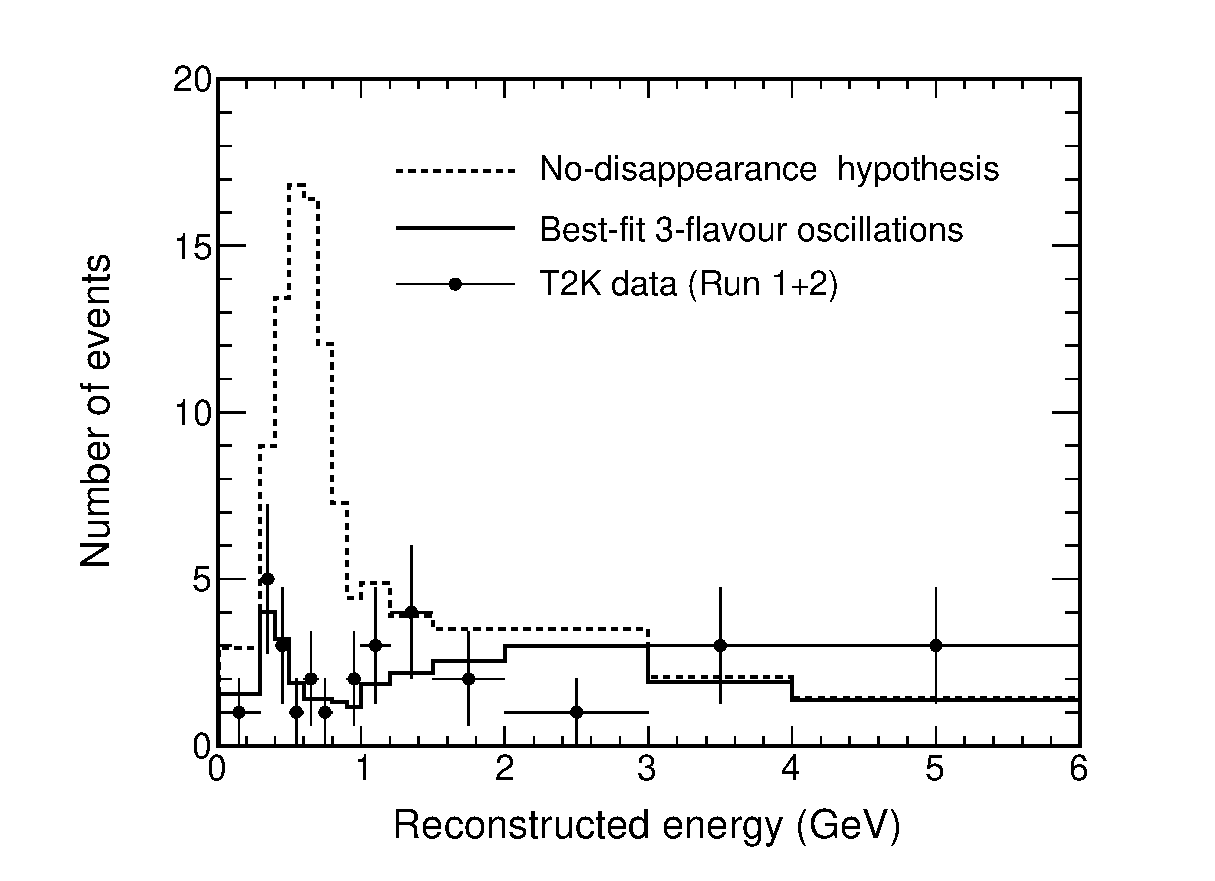
\includegraphics{./images/best_fit/SKErecoNullBestFitGenie.eps}}
\caption[Reconstructed energy spectrum of the 31 Run 1+2 data events compared with the expected spectra in Super-K without disappearance and
with best-fit 3-flavour oscillations (GENIE)]
{Reconstructed energy spectrum of the 31 Run 1+2 data events compared with the expected spectra in Super-K without disappearance and 
with best-fit 3-flavour oscillations (GENIE); the spectrum for best-fit oscillations uses $\sin^{2}(2 \theta_{12})$ = 0.87, $\sin^{2}(2 \theta_{13})$ = 0.1,
$\Delta m_{21}^{2}$ = 7.6 $\times 10^{-5}$ eV$^{2}$/c$^{4}$, $\delta_{CP}$ = 0 and Earth crust density = 2.6 g/cm$^{3}$. The atmospheric $\Delta m^{2}$ is input 
as $|\Delta m_{32}^{2}|$. A variable binning scheme is used here for the purpose of illustration only; the actual analysis used equal-sized 50 MeV bins.}
\label{bestfitdataexpectedgenie}
\end{center}
\end{figure}

\begin{figure}
\begin{center}
\resizebox{13cm}{!}{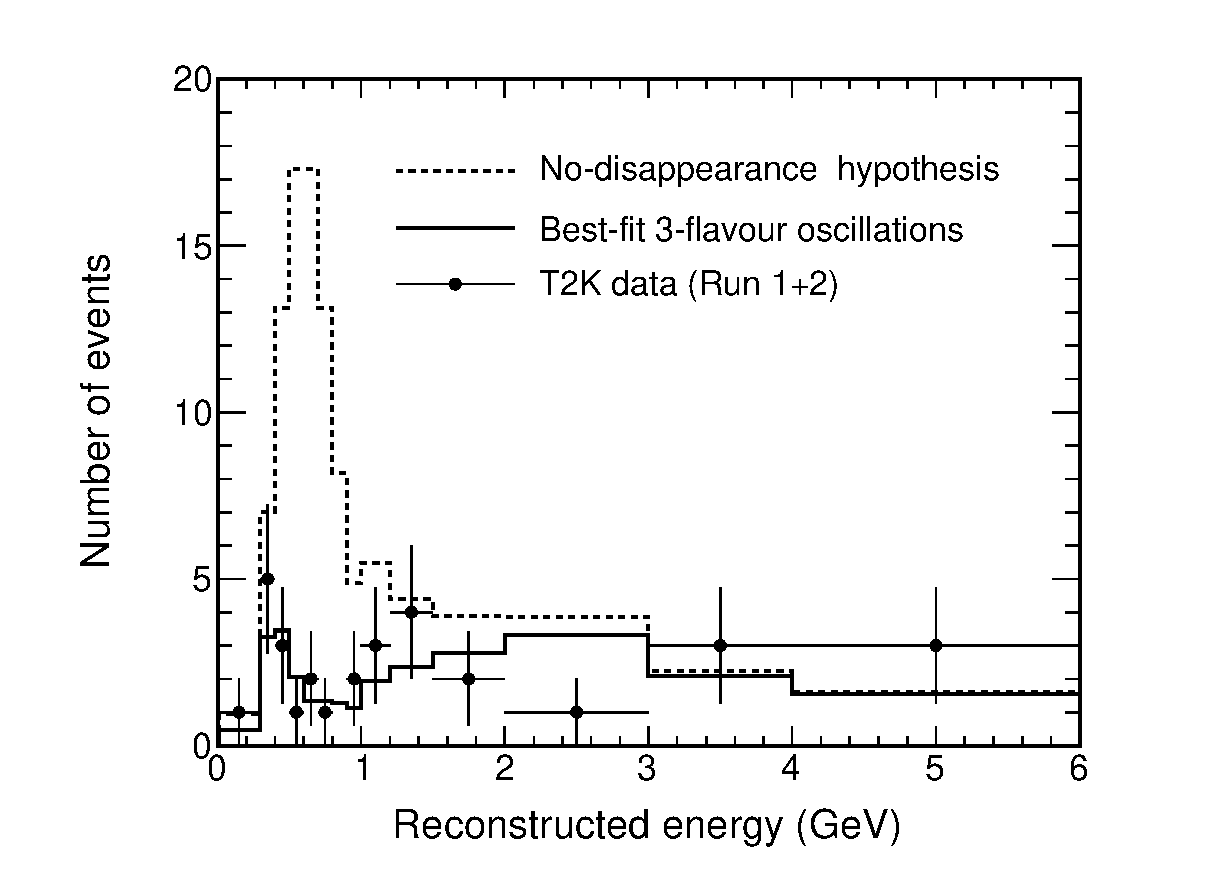
\includegraphics{./images/best_fit/SKErecoNullBestFitNeut.eps}}
\caption[Reconstructed energy spectrum of the 31 Run 1+2 data events compared with the expected spectra in Super-K without disappearance and
with best-fit 3-flavour oscillations (NEUT)]
{Reconstructed energy spectrum of the 31 Run 1+2 data events compared with the expected spectra in Super-K without disappearance and
with best-fit 3-flavour oscillations (NEUT); the spectrum for best-fit oscillations uses $\sin^{2}(2 \theta_{12})$ = 0.87, $\sin^{2}(2 \theta_{13})$ = 0.1,
$\Delta m_{21}^{2}$ = 7.6 $\times 10^{-5}$ eV$^{2}$/c$^{4}$, $\delta_{CP}$ = 0 and Earth crust density = 2.6 g/cm$^{3}$. The atmospheric $\Delta m^{2}$ is input
as $|\Delta m_{32}^{2}|$. A variable binning scheme is used here for the purpose of illustration only; the actual analysis used equal-sized 50 MeV bins.}
\label{bestfitdataexpectedneut}
\end{center}
\end{figure}

\begin{figure}
\begin{center}
\resizebox{13cm}{!}{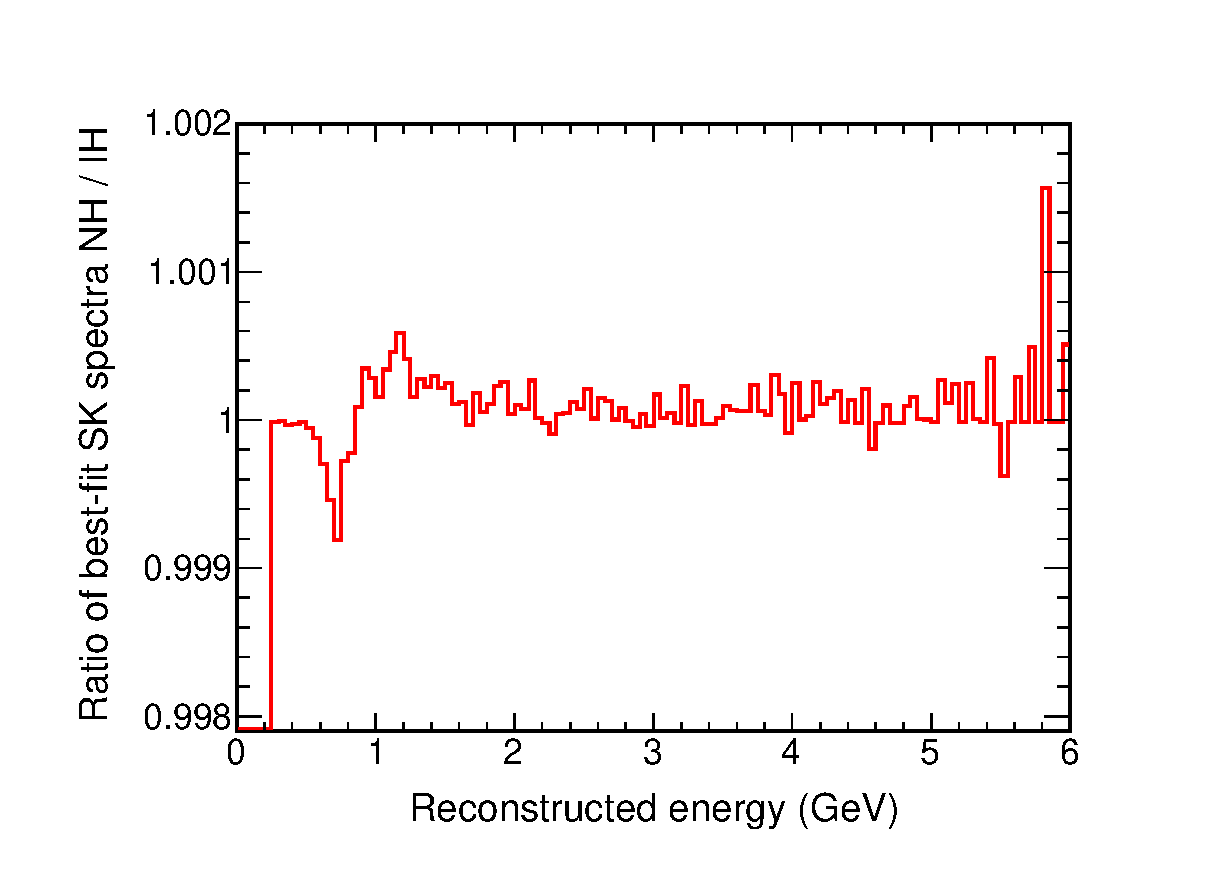
\includegraphics{./images/best_fit/BestFitRatioNormalInverted.eps}}
\caption[Ratio of best-fit 3-flavour reconstructed Super-K energy spectrum assuming the normal mass
hierarchy to that assuming the inverted mass hierarchy using NEUT]
{Ratio of best-fit 3-flavour reconstructed Super-K energy spectrum assuming the normal mass
hierarchy to that assuming the inverted mass hierarchy using NEUT; $\sin^{2}(2 \theta_{12})$ = 0.87, $\sin^{2}(2 \theta_{13})$ = 0.1,
$\Delta m_{21}^{2}$ = 7.6 $\times 10^{-5}$ eV$^{2}$/c$^{4}$, $\delta_{CP}$ = 0 and Earth crust density = 2.6 g/cm$^{3}$. The atmospheric 
$\Delta m^{2}$ is input as $|\Delta m_{32}^{2}|$.}
\label{rationormalinverted}
\end{center}
\end{figure}

\begin{figure}
\begin{center}
\resizebox{13cm}{!}{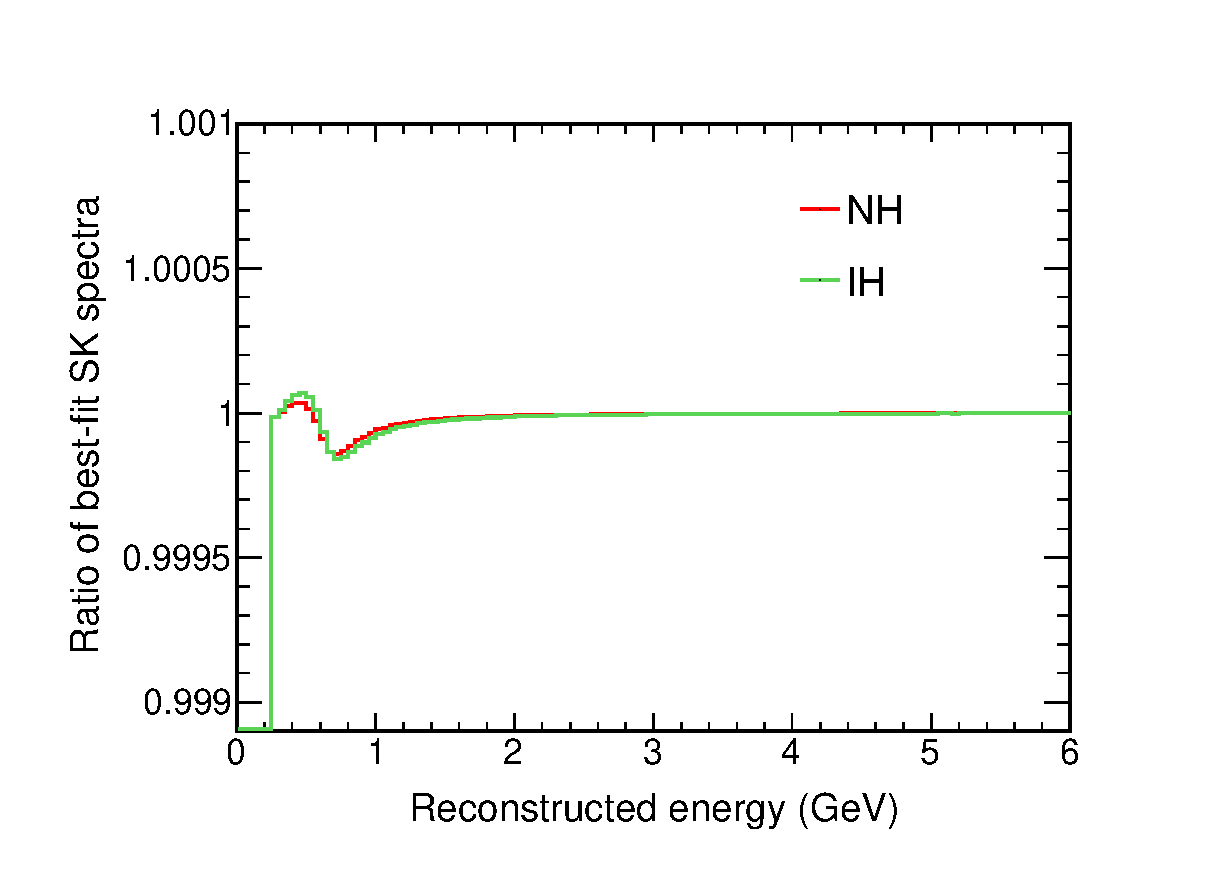
\includegraphics{./images/best_fit/BestFitRatioFogliLisi.eps}}
\caption[Ratio of best-fit 3-flavour reconstructed Super-K energy spectrum for the atmospheric $\Delta m^{2}$ input as $|\Delta m_{32}^{2}|$ to
the best-fit spectrum for the atmospheric $\Delta m^{2}$ input as $|\Delta m_{FL}^{2}|$ using NEUT]
{Ratio of best-fit 3-flavour reconstructed Super-K energy spectrum for the atmospheric $\Delta m^{2}$ input as $|\Delta m_{32}^{2}|$ to 
the best-fit spectrum for the atmospheric $\Delta m^{2}$ input as $|\Delta m_{FL}^{2}|$ = $|m_{3}^{2} - [(m_{2}^{2} + m_{1}^{2}) / 2]|$ using NEUT; 
$\sin^{2}(2 \theta_{12})$ = 0.87, $\sin^{2}(2 \theta_{13})$ = 0.1, $\Delta m_{21}^{2}$ = 7.6 $\times 10^{-5}$ eV$^{2}$/c$^{4}$, $\delta_{CP}$ = 0, Earth
crust density = 2.6 g/cm$^{3}$, NH = normal mass hierarchy, IH = inverted mass hierarchy.}
\label{ratiofoglilisi}
\end{center}
\end{figure}

The uncertainties in the best-fit values of $\sin^{2}(2 \theta_{23})$ and $|\Delta m_{32}^{2}|$ due to uncertainties in 
the values of the non-23 oscillation parameters were estimated by creating 50000 fake datasets for each mass 
hierarchy. These fake datasets did not include statistical fluctuations, and they were made using random input values of 
$\sin^{2}(2 \theta_{12})$, $\sin^{2}(2 \theta_{13})$ and $\Delta m_{21}^{2}$ drawn from Gaussian distributions with means 
equal to the nominal values and standard deviations equal to the 1$\sigma$ errors. The uncertainties in $\sin^{2}(2 \theta_{12})$ 
and $\Delta m_{21}^{2}$ are taken from KamLAND combined with solar experiments \cite{Kamland}, while those in 
$\sin^{2}(2 \theta_{13})$ are computed as a weighted average of measurements from Daya Bay \cite{DayaBay} and Reno \cite{Reno}. 
The input values of $\delta_{CP}$ were randomly drawn from a uniform distribution between -$\pi$ and +$\pi$. The input value of 
$\sin^{2}(2 \theta_{23})$ was fixed at 0.9 (to allow an estimate of both plus and minus uncertainties) and the input value of 
$|\Delta m_{32}^{2}|$ was fixed at 2.32 $\times$ 10$^{-3}$ eV$^{2}$/c$^{4}$. 

When fitting the fake datasets to obtain the best-fit points, the expected numbers of single $\mu$-like ring events in Super-K 
with oscillations were again calculated with fixed values of $\sin^{2}(2 \theta_{12})$, $\sin^{2}(2 \theta_{13})$, $\Delta m_{21}^{2}$ and $\delta_{CP}$, 
while $\sin^{2}(2 \theta_{23})$ and $|\Delta m_{32}^{2}|$ were allowed to vary in order to find their best-fit values. When all the non-23 
parameters were varied together, the standard deviations of the best-fit values of $\sin^{2}(2 \theta_{23})$ were 0.5\% (NH) and 0.4\% 
(IH), and those of the best-fit values of $|\Delta m_{32}^{2}|$ were 0.7\% (NH) and 0.4\% (IH). Additional fake datasets were made in which 
only one non-23 parameter was varied at a time, with the other parameters being fixed at their default values. The results are given in table 
\ref{bestfitnon23errors} which shows that the non-23 uncertainties in the best-fit points are almost entirely due to uncertainties in $\delta_{CP}$.
As a comparison, the uncertainties in the best-fit points due to the combined systematic uncertainties were considerably larger at 4.3\% (NH) 
and 4.9\% (IH) for $\sin^{2}(2 \theta_{23})$ and 4.8\% (NH) and 5.1\% (IH) for $|\Delta m_{32}^{2}|$. 

\begin{table}
\caption[Uncertainties in the best-fit values of $\sin^{2}(2 \theta_{23})$ and $|\Delta m_{32}^{2}|$ due to uncertainties in the non-23
oscillation parameters using NEUT]
{Uncertainties in the best-fit values of $\sin^{2}(2 \theta_{23})$ and $|\Delta m_{32}^{2}|$ due to uncertainties in the non-23 
oscillation parameters using NEUT. These are varied using random numbers drawn from Gaussian distributions with means equal to the nominal values and 
standard deviations equal to the 1$\sigma$ errors, except for $\delta_{CP}$ which is varied using a random number drawn from a uniform 
distribution between -$\pi$ and +$\pi$. When fixed these parameters have the values $\sin^{2}(2 \theta_{12})$ = 0.87, $\sin^{2}(2 \theta_{13})$ 
= 0.1, $\Delta m_{21}^{2}$ = 7.6 $\times$ 10$^{-5}$ eV$^{2}$/c$^{4}$, $\delta_{CP}$ = 0. The Earth crust density is taken to be 2.6 g/cm$^{3}$, and NH = 
normal mass hierarchy, IH = inverted mass hierarchy.}
\centering
\begin{tabular}{| c | c | c | c | c |}
\hline
Parameter & Uncertainty & Uncertainty & Uncertainty & Uncertainty \\
 & in $\sin^{2}(2 \theta_{23})$ & in $|\Delta m_{32}^{2}|$ & in $\sin^{2}(2 \theta_{23})$ & in $|\Delta m_{32}^{2}|$ \\
 & (NH) & (NH) & (IH) & (IH) \\
\hline
$\sin^{2}(2 \theta_{13})$ & 0.08\% & 0.2\% & 0.01\% & 0.05\%\\
\hline
$\delta_{CP}$ & 0.5\% & 0.6\% &  0.35\% & 0.4\%\\
\hline
$\sin^{2}(2 \theta_{12})$ & 0.004\% & 0.09\% & 0.007\% & 0.09\%\\
\hline
$\Delta m_{21}^{2}$ & 0.01\% & 0.04\% & 0.009\%  & 0.05\%\\
\hline
All non-23 parameters & 0.5\% & 0.7\% & 0.4\% & 0.4\%\\
\hline
All systematics & 4.3\% & 4.8\% & 4.9\% & 5.1\%\\
\hline
\end{tabular}
\label{bestfitnon23errors}
\end{table}

In order to show these uncertainties in the best-fit points graphically, they were also estimated by varying each non-23 parameter 
by $\pm$1$\sigma$ in a single toy experiment without statistical fluctuations. Once more the input value of $\sin^{2}(2 \theta_{23})$ was fixed 
at 0.9 and the input value of $|\Delta m_{32}^{2}|$ was fixed at 2.32 $\times$ 10$^{-3}$ eV$^{2}$/c$^{4}$. The results are shown in figure \ref{bestfitstarplot}, 
and the uncertainties in the best-fit points are again almost entirely due to uncertainties in $\delta_{CP}$.

\begin{figure}
\begin{center}
\resizebox{11cm}{!}{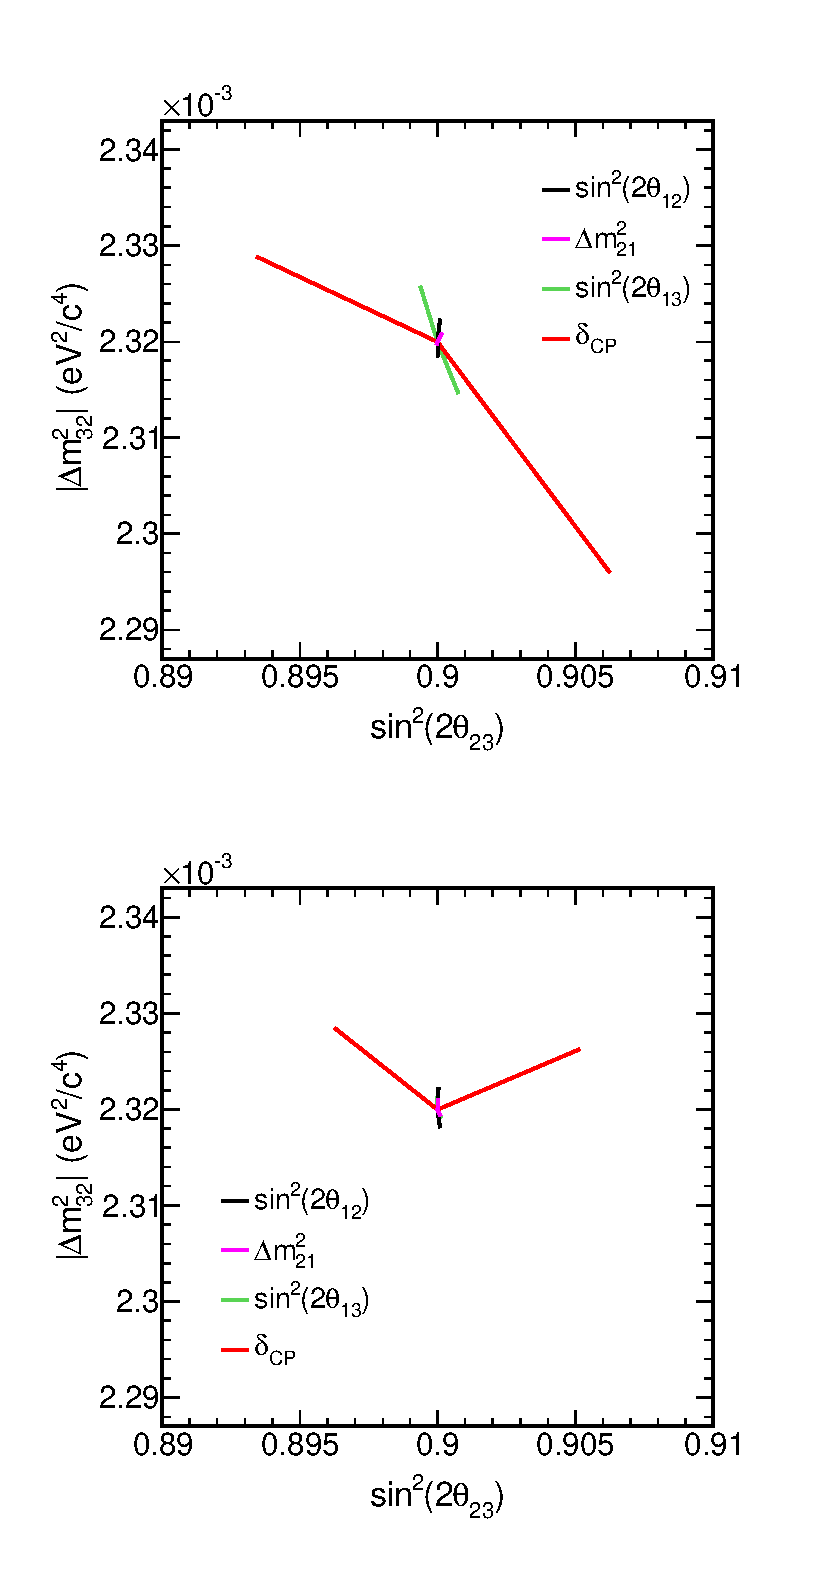
\includegraphics{./images/best_fit/BestFitStarPlot.eps}}
\caption[Uncertainties in the best-fit values of $\sin^{2}(2 \theta_{23})$ and $|\Delta m_{32}^{2}|$ due to uncertainties in the non-23
oscillation parameters for the normal mass hierarchy (top) and the inverted mass hierarchy (bottom) using NEUT]
{Uncertainties in the best-fit values of $\sin^{2}(2 \theta_{23})$ and $|\Delta m_{32}^{2}|$ due to uncertainties in the non-23 
oscillation parameters for the normal mass hierarchy (top) and the inverted mass hierarchy (bottom) using NEUT; uncertainties in $\delta_{CP}$ are shown 
for changes from 0 to +$\pi$/2 and -$\pi$/2.}
\label{bestfitstarplot}
\end{center}
\end{figure}

Since it is not curremtly possible to define a $\pm$1$\sigma$ error in $\delta_{CP}$, the effects of varying it on the best-fit values of 
$\sin^{2}(2 \theta_{23})$ and $|\Delta m_{32}^{2}|$ are plotted in figure \ref{bestfitstarplotdeltacp}. $\delta_{CP}$ can affect $|\Delta m_{32}^{2}|$ 
only (for example if it changes from 0.0 to $\pi$) or $\sin^{2}(2 \theta_{23})$ only (for example if it changes from 0.0 to $\frac{3\pi}{4}$) or 
both (for example if it changes from 0.0 to $\frac{\pi}{2}$).

\begin{figure}
\begin{center}
\resizebox{11cm}{!}{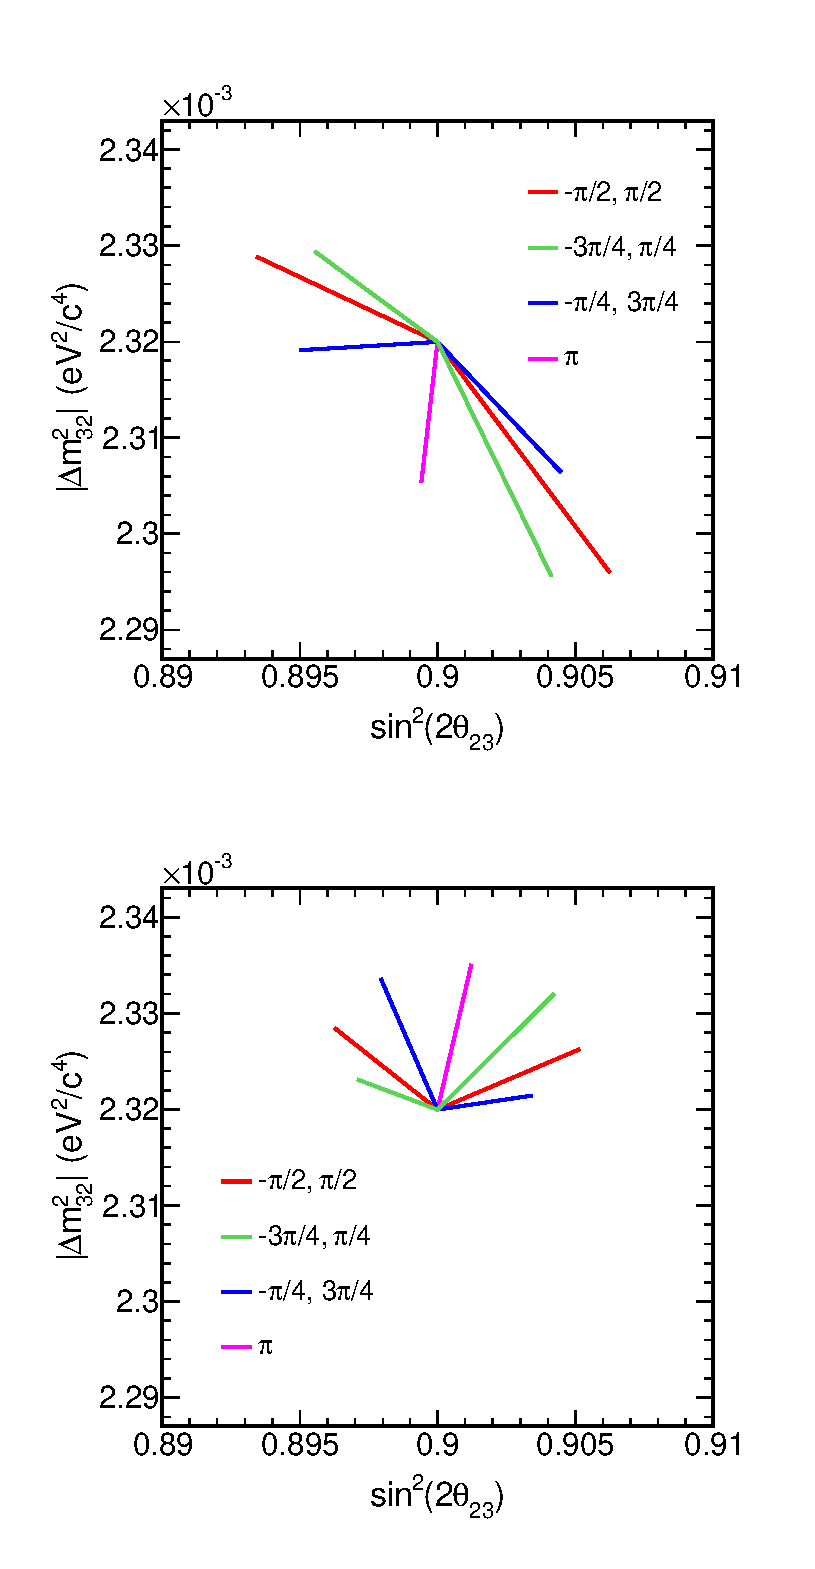
\includegraphics{./images/best_fit/BestFitStarPlotDeltaCP.eps}}
\caption{Uncertainties in the best-fit values of $\sin^{2}(2 \theta_{23})$ and $|\Delta m_{32}^{2}|$ due to uncertainties in $\delta_{CP}$ for the 
normal mass hierarchy (top) and the inverted mass hierarchy (bottom) using NEUT}
\label{bestfitstarplotdeltacp}
\end{center}
\end{figure}

\clearpage

\section{3-flavour $\nu_{\mu}$-disappearance confidence contours for the Run 1+2 dataset}
\label{sec:conf_regions}

Confidence contours for the oscillation parameters $\sin^{2}(2 \theta_{23})$ and $|\Delta m_{32}^{2}|$ are drawn using the method 
of Feldman and Cousins \cite{FeldmanCousins}. Details of its implementation in the $\nu_{\mu}$-disappearance analysis are given in 
section 3.4 in \cite{OurRun1DisappAnalysis2F}.

A comparison of the stat + syst 68\% and 90\% confidence regions between the 2-flavour \cite{OurRun1and2Analysis2F} and 3-flavour 
analyses is shown using GENIE in figure \ref{contours3flavourgenie} and using NEUT in figure \ref{contours3flavourneut}. In these 
figures the non-23 oscillation parameters are fixed. The 3-flavour contours are 
narrower in $\sin^{2}(2 \theta_{23})$ than the 2-flavour contours, and this is because the 3-flavour best-fit points are nearer to 
$\sin^{2}(2 \theta_{23})$ = 1.0 than the 2-flavour best-fit points. The 3-flavour contours for the IH include higher values of 
$|\Delta m_{32}^{2}|$ than those for the NH it is necessary to choose a higher value of $|\Delta m_{32}^{2}|$ for the IH than for the NH 
in order to fit the oscillation dip at a certain energy in the real data.

It was found that uncertainties in the non-23 oscillation parameters had a neglible effect on the 3-flavour confidence contours. This was 
checked by creating 10000 toy MC experiments using NEUT for each of a few oscillation parameter points on or near the 3-flavour 68\% and 90\% 
contours for the NH only. Examples of the cumulative distributions of $\Delta\chi^{2}$ are given for a point on the physical 
boundary in figure \ref{cumdeltachisq100310} and a point away from the physical boundary in figure \ref{cumdeltachisq087240}. In both 
cases the distributions including the non-23 uncertainties are negligibly different from those without them. For this reason, it was decided 
not to remake the Feldman-Cousins contours including the non-23 uncertainties for the whole grid of oscillation parameter points for this 
analysis. However in future analyses by the Rutherford-Oxford-Lancs group, the uncertainties in the non-23 oscillation parameters \emph{will} 
be taken into account in the confidence contours.

A comparison of the 90\% 3-flavour confidence contours with previous results from MINOS \cite{Minos2011} and Super-K \cite{OldDisappSuperK} 
is also given using GENIE in figure \ref{contours90plusexternalgenie} and using NEUT in figure \ref{contours90plusexternalneut}.

\begin{figure}
\begin{center}
\resizebox{13cm}{!}{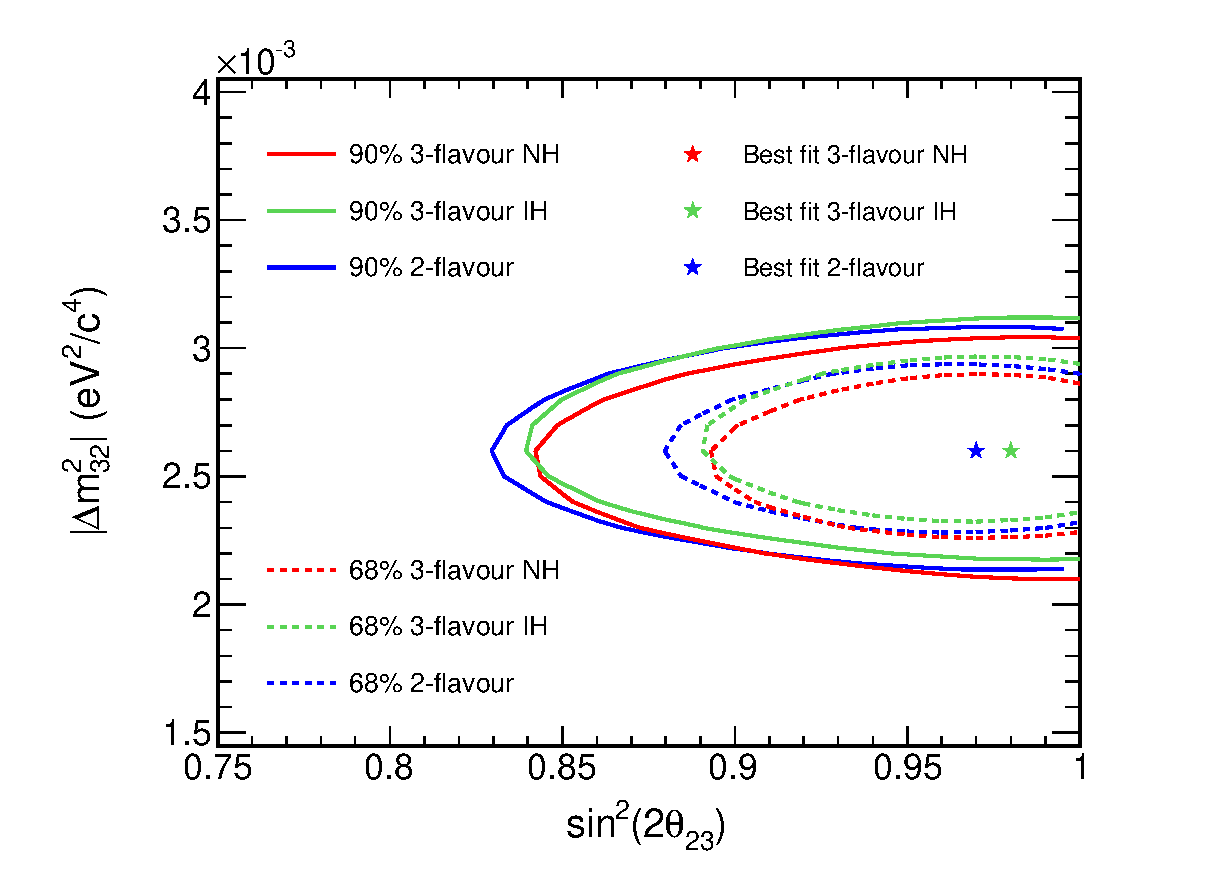
\includegraphics{./images/confidence_contours/ConfidenceContours3FlavourGenie.eps}}
\caption[Comparison of confidence contours for $\sin^{2}(2 \theta_{23})$ and $|\Delta m_{32}^{2}|$ between 2-flavour, 3-flavour (NH)
and 3-flavour (IH) using GENIE]
{Comparison of confidence contours for $\sin^{2}(2 \theta_{23})$ and $|\Delta m_{32}^{2}|$ between 2-flavour, 3-flavour (NH) 
and 3-flavour (IH) using GENIE; the 3-flavour best-fit points are identical for the NH and IH. All contours include both statistical and 
systematic uncertainties. The non-23 oscillation parameters are fixed.}
\label{contours3flavourgenie}
\end{center}
\end{figure}

\begin{figure}
\begin{center}
\resizebox{13cm}{!}{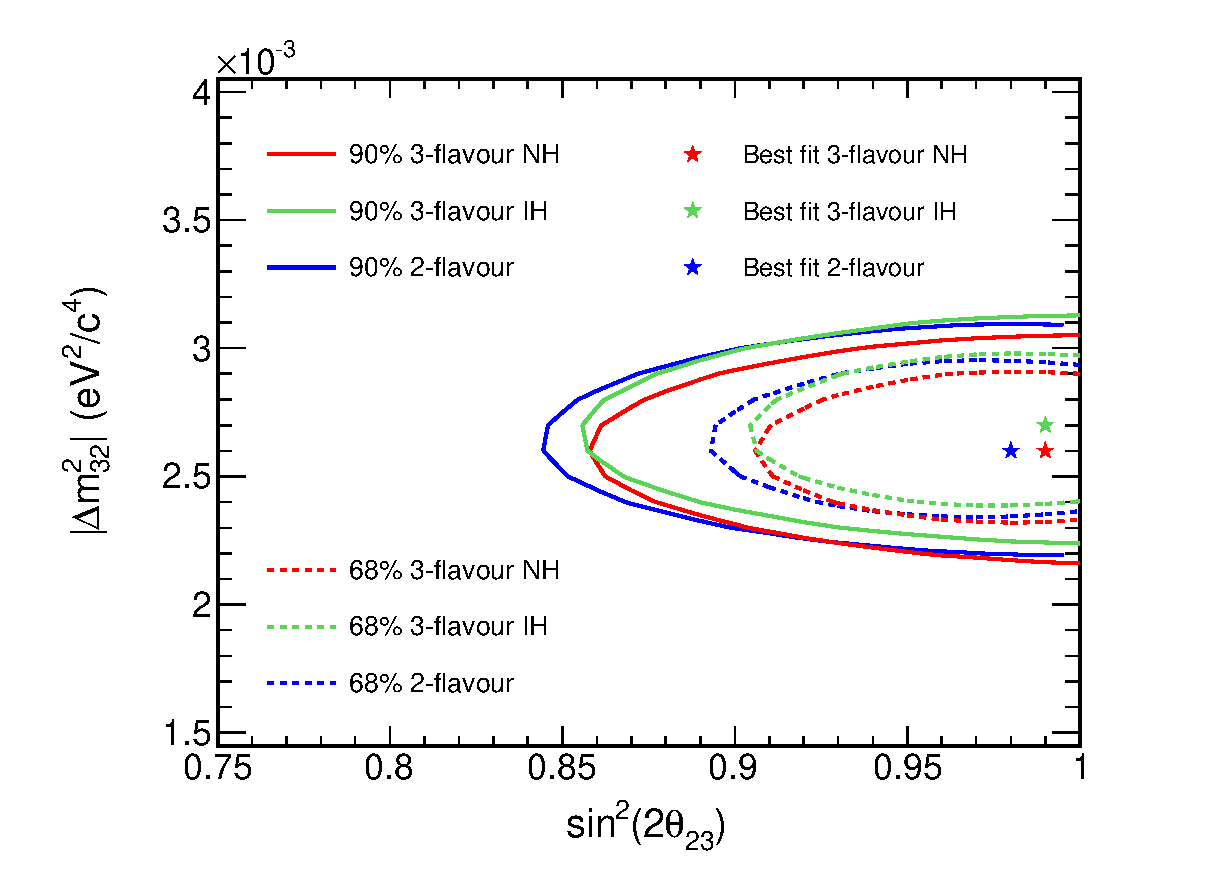
\includegraphics{./images/confidence_contours/ConfidenceContours3FlavourNeut.eps}}
\caption[Comparison of confidence contours for $\sin^{2}(2 \theta_{23})$ and $|\Delta m_{32}^{2}|$ between 2-flavour, 3-flavour (NH)
and 3-flavour (IH) using NEUT]
{Comparison of confidence contours for $\sin^{2}(2 \theta_{23})$ and $|\Delta m_{32}^{2}|$ between 2-flavour, 3-flavour (NH)
and 3-flavour (IH) using NEUT. All contours include both statistical and systematic uncertainties. The non-23 oscillation parameters 
are fixed.}
\label{contours3flavourneut}
\end{center}
\end{figure}

\begin{figure}
\begin{center}
\resizebox{11cm}{!}{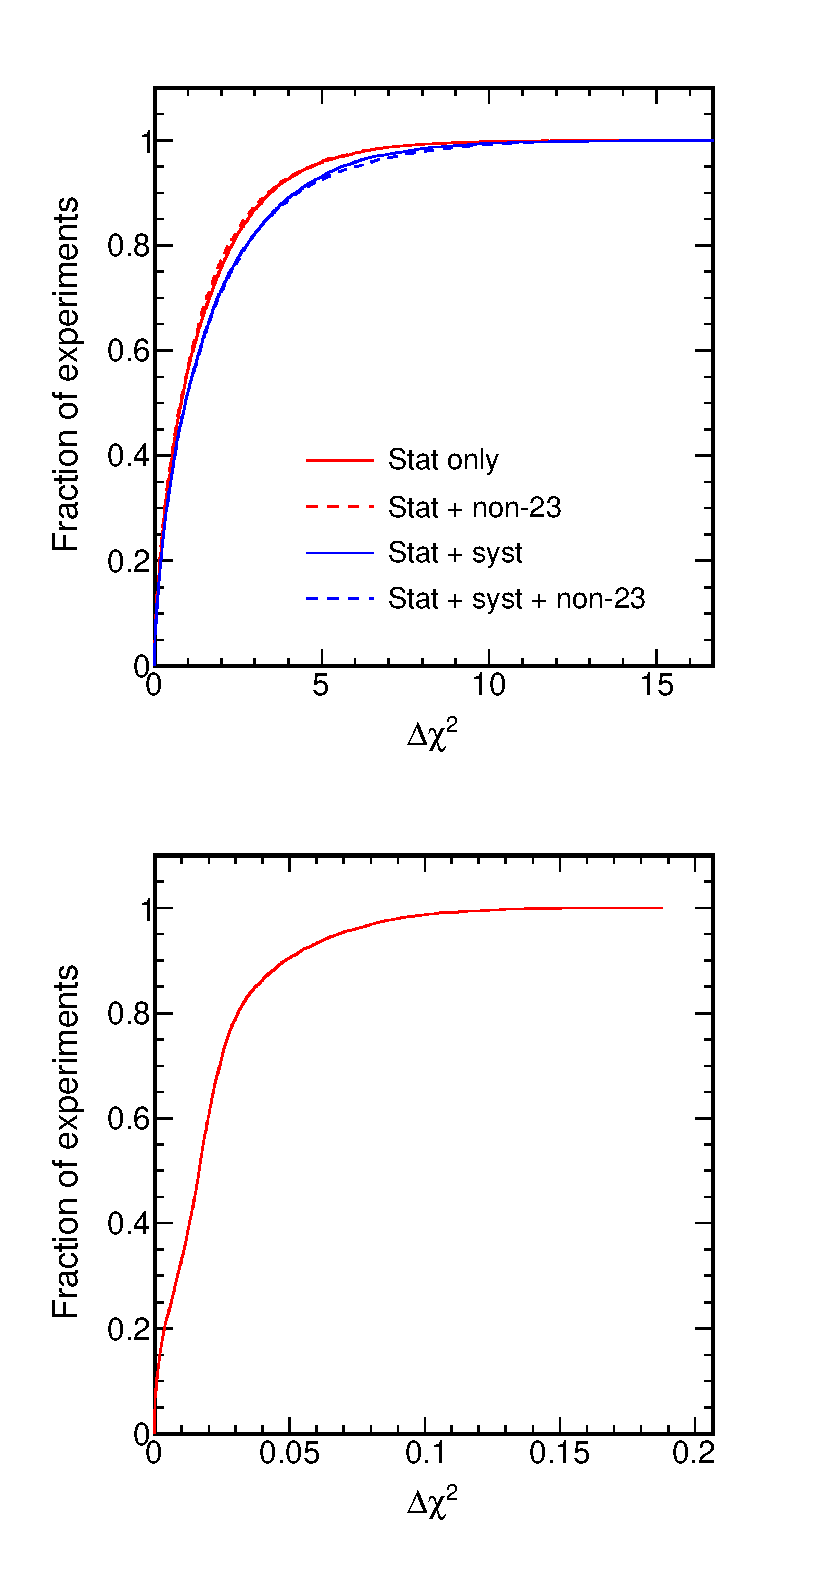
\includegraphics{./images/confidence_contours/DeltaChisqCritWithNon23_100_310.eps}}
\caption[Cumulative distributions of $\Delta\chi^{2}$ (= $\chi^{2}_{TRUE}$ - $\chi^{2}_{BESTFIT}$) for 10000 toy MC experiments created
at true values of $\sin^{2}(2 \theta_{23})$ = 1.0 and $|\Delta m_{32}^{2}|$ = 3.1 $\times$ 10$^{-3}$ eV$^{2}$/c$^{4}$ using NEUT]
{Cumulative distributions of $\Delta\chi^{2}$ (= $\chi^{2}_{TRUE}$ - $\chi^{2}_{BESTFIT}$) for 10000 toy MC experiments created 
at true values of $\sin^{2}(2 \theta_{23})$ = 1.0 and $|\Delta m_{32}^{2}|$ = 3.1 $\times$ 10$^{-3}$ eV$^{2}$/c$^{4}$ using NEUT; stat only, stat 
+ non-23, stat + syst and stat + syst + non-23 (top) and non-23 only (bottom). Normal mass hierarchy, Earth crust density = 2.6 g/cm$^{3}$. 
When not varied, the non-23 oscillation parameters are fixed at $\sin^{2}(2 \theta_{12})$ = 0.87, $\sin^{2}(2 \theta_{13})$ = 0.1, 
$\Delta m_{21}^{2}$ = 7.6 $\times$ 10$^{-5}$ eV$^{2}$/c$^{4}$, $\delta_{CP}$ = 0.}
\label{cumdeltachisq100310}
\end{center}
\end{figure}

\begin{figure}
\begin{center}
\resizebox{11cm}{!}{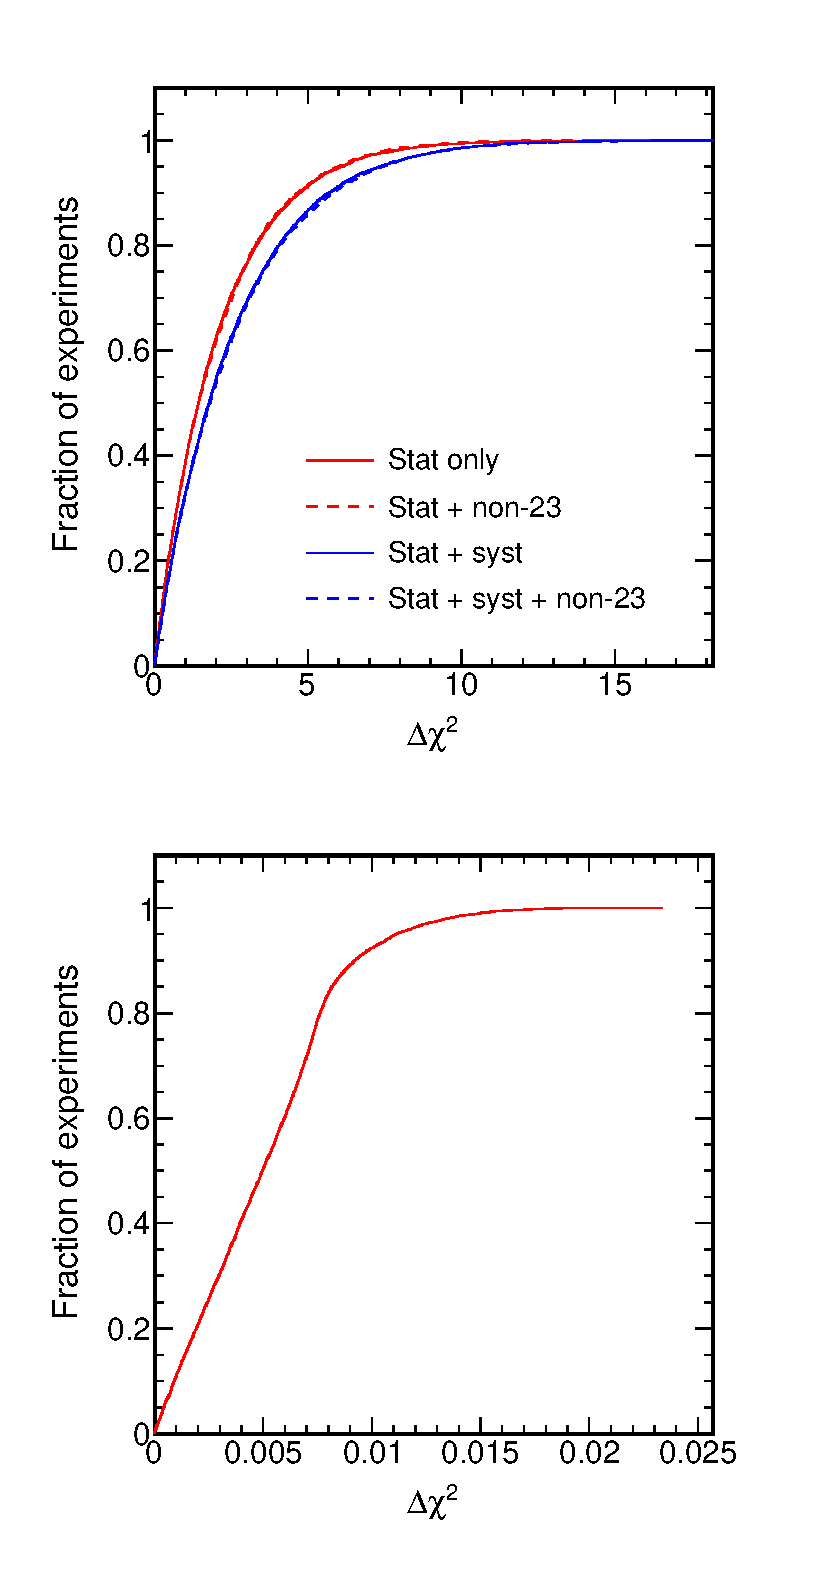
\includegraphics{./images/confidence_contours/DeltaChisqCritWithNon23_087_240.eps}}
\caption[Cumulative distributions of $\Delta\chi^{2}$ (= $\chi^{2}_{TRUE}$ - $\chi^{2}_{BESTFIT}$) for 10000 toy MC experiments created
at true values of $\sin^{2}(2 \theta_{23})$ = 0.87 and $|\Delta m_{32}^{2}|$ = 2.4 $\times$ 10$^{-3}$ eV$^{2}$/c$^{4}$ using NEUT]
{Cumulative distributions of $\Delta\chi^{2}$ (= $\chi^{2}_{TRUE}$ - $\chi^{2}_{BESTFIT}$) for 10000 toy MC experiments created
at true values of $\sin^{2}(2 \theta_{23})$ = 0.87 and $|\Delta m_{32}^{2}|$ = 2.4 $\times$ 10$^{-3}$ eV$^{2}$/c$^{4}$ using NEUT; stat only, stat 
+ non-23, stat + syst and stat + syst + non-23 (top) and non-23 only (bottom). Normal mass hierarchy, Earth crust density = 2.6 g/cm$^{3}$. 
When not varied, the non-23 oscillation parameters are fixed at $\sin^{2}(2 \theta_{12})$ = 0.87, $\sin^{2}(2 \theta_{13})$ = 0.1, 
$\Delta m_{21}^{2}$ = 7.6 $\times$ 10$^{-5}$ eV$^{2}$/c$^{4}$, $\delta_{CP}$ = 0.}
\label{cumdeltachisq087240}
\end{center}
\end{figure}

\begin{figure}
\begin{center}
\resizebox{13cm}{!}{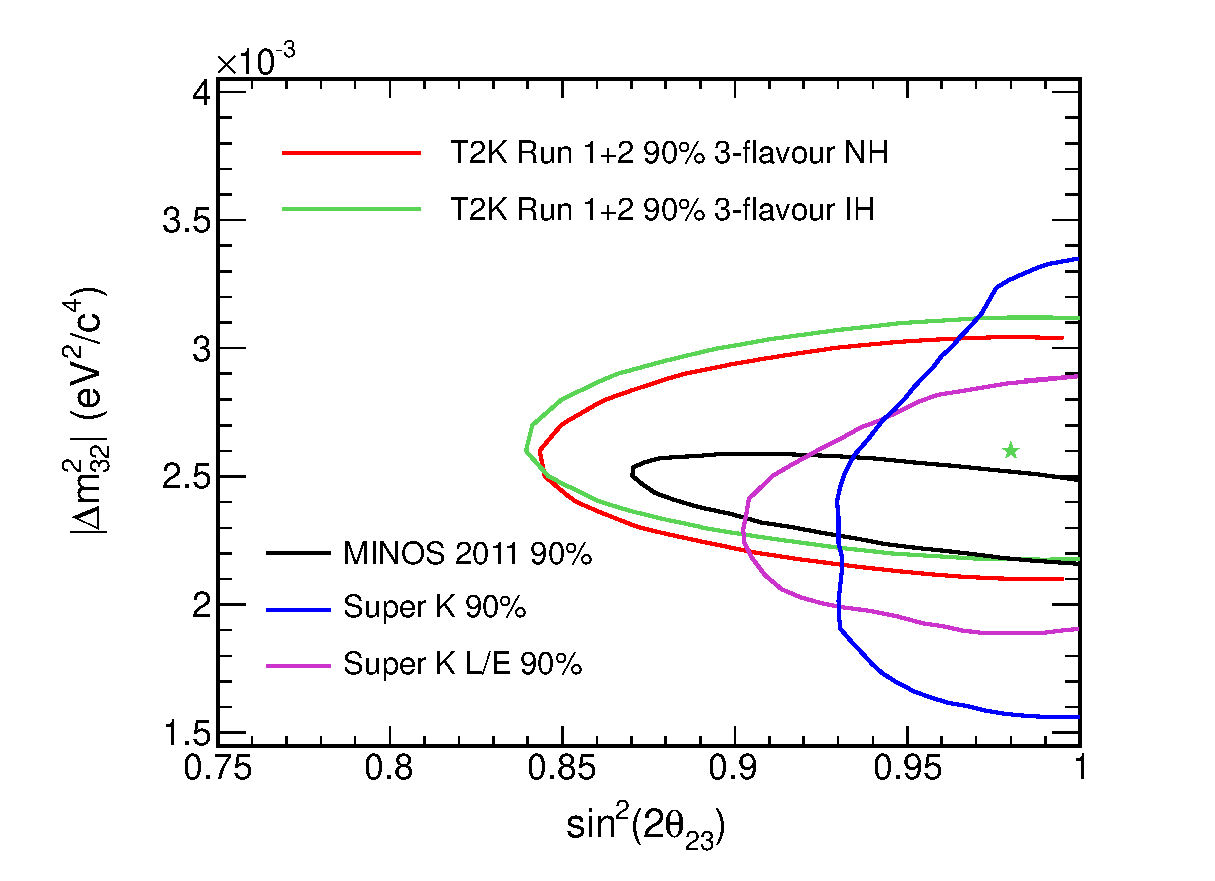
\includegraphics{./images/confidence_contours/ConfidenceContoursPlusExternalGenie.eps}}
\caption[Comparison of T2K Run 1+2 3-flavour 90\% confidence contours for $\sin^{2}(2 \theta_{23})$ and $|\Delta m_{32}^{2}|$ (GENIE) with
results from MINOS \cite{Minos2011} and Super-K \cite{OldDisappSuperK}]
{Comparison of T2K Run 1+2 3-flavour 90\% confidence contours for $\sin^{2}(2 \theta_{23})$ and $|\Delta m_{32}^{2}|$ (GENIE) with 
results from MINOS \cite{Minos2011} and Super-K \cite{OldDisappSuperK}; the T2K 3-flavour best-fit points are identical for the NH and IH.}
\label{contours90plusexternalgenie}
\end{center}
\end{figure}

\begin{figure}
\begin{center}
\resizebox{13cm}{!}{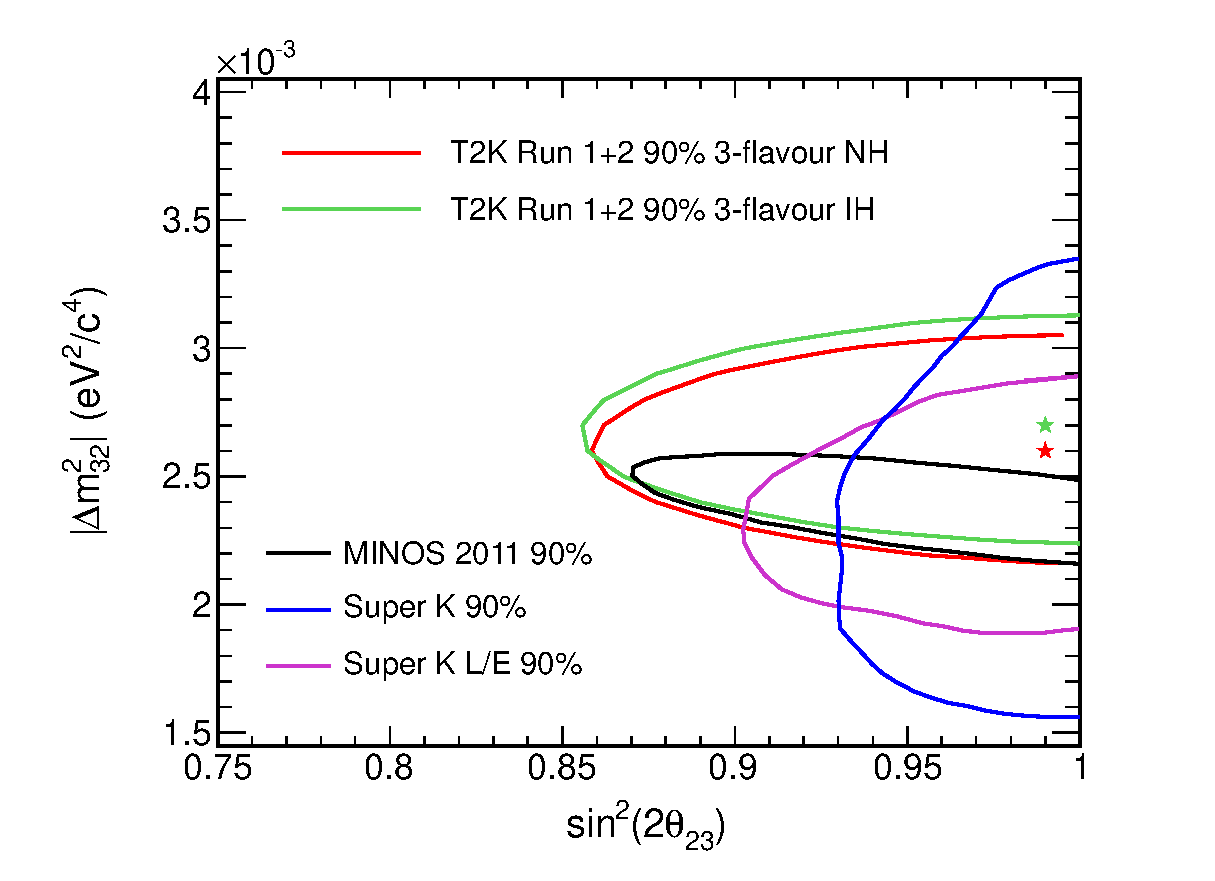
\includegraphics{./images/confidence_contours/ConfidenceContoursPlusExternalNeut.eps}}
\caption{Comparison of T2K Run 1+2 3-flavour 90\% confidence contours for $\sin^{2}(2 \theta_{23})$ and $|\Delta m_{32}^{2}|$ (NEUT) with
results from MINOS \cite{Minos2011} and Super-K \cite{OldDisappSuperK}}
\label{contours90plusexternalneut}
\end{center}
\end{figure}

\clearpage 

\section {Summary }
\label{sec:summary}

In this note, we have presented the results of a 3-flavour $\nu_{\mu}$-disappearance analysis 
on the combined Run 1+2 dataset, which corresponds to an integrated J-PARC neutrino beam exposure 
of 1.431 $\times$ 10$^{20}$ POT. The analysis method was identical to that used in our earlier analysis
reported in Ref.\ \cite{OurRun1and2Analysis2F} except that 3-flavour oscillation probabilities were 
used instead of the 2-flavour approximation and oscillated $\nu_{e}$ templates were added in the interaction 
modes CCQE, CC1$\pi$ and CC other. 

In the 3-flavour analysis, the total predicted number of single $\mu$-like ring events in Super-K is higher 
for the inverted hierarchy (IH) than for the normal hierarchy (NH) when the atmospheric mass-squared difference 
is $|\Delta m^{2}_{32}|$. This is because more events are predicted above the oscillation maximum for the IH than 
for the NH and less are predicted below it. In turn this is due to the 3-flavour $\nu_{\mu}$-survival probability 
being higher for the IH than the NH above the oscillation maximum and lower below the oscillation maximum. Since 
there are more events above the oscillation maximum than below it, the total predicted number is higher for the 
IH than for the NH. This is true for any combination of the non-23 oscillation parameters. 

Uncertainties in $\delta_{CP}$ can change the predicted reconstructed spectrum of single $\mu$-like ring events 
in Super-K by up to 5\% above the oscillation maximum and by up to 3\% below it. This is larger than changes 
in the spectrum due to uncertainties in $\sin^{2}(2 \theta_{13})$, $\sin^{2}(2 \theta_{12})$ and $\Delta m_{21}^{2}$ 
which are $\leq$ 0.5\%.

A 3-flavour $\nu_{\mu}$-disappearance fit was made of the observed Super-K reconstructed energy spectrum of 
single $\mu$-like ring events in the combined Run 1+2 dataset. In this fit, sin$^{2}$(2$\theta_{23}$) and 
$|\Delta m^{2}_{32}|$ were varied to find their best-fit values, but the non-23 oscillation parameters were 
fixed. Using GENIE, this gave best-fit values of 
sin$^{2}$(2$\theta_{23}$) = 0.98, $|\Delta m^{2}_{32}|$ = 2.6 $\times$ 10$^{-3}$ eV$^{2}$/c$^{4}$ for both mass 
hierarchies, while a fit using NEUT gave sin$^{2}$(2$\theta_{23}$) = 0.99, $|\Delta m^{2}_{32}|$ 
= 2.6 $\times$ 10$^{-3}$ eV$^{2}$/c$^{4}$ for the NH and sin$^{2}$(2$\theta_{23}$) = 0.99, $|\Delta m^{2}_{32}|$
= 2.7 $\times$ 10$^{-3}$ eV$^{2}$/c$^{4}$ for the IH. For comparison, the best-fit values from the 2-flavour 
analysis in \cite{OurRun1and2Analysis2F} were sin$^{2}$(2$\theta_{23}$) = 0.97, $|\Delta m^{2}_{32}|$ 
= 2.6 $\times$ 10$^{-3}$ eV$^{2}$/c$^{4}$ using GENIE and sin$^{2}$(2$\theta_{23}$) = 0.98, $|\Delta m^{2}_{32}|$ 
= 2.6 $\times$ 10$^{-3}$ eV$^{2}$/c$^{4}$ using NEUT. The 3-flavour best-fit points were higher in sin$^{2}$(2$\theta_{23}$) 
than those in the 2-flavour analysis due to the effect of sin$^{2}$(2$\theta_{13}$): in the 3-flavour analysis 
sin$^{2}$(2$\theta_{13}$) = 0.1, whereas in the 2-flavour analysis the approximation sin$^{2}$(2$\theta_{13}$) 
= 0 was used.

Uncertainties in the best-fit points due to uncertainties in $\delta_{CP}$ are larger than those due to 
uncertainties in $\sin^{2}(2 \theta_{13})$, $\sin^{2}(2 \theta_{12})$ and $\Delta m_{21}^{2}$; these uncertainties 
due to $\delta_{CP}$ are 0.5\% (NH) and 0.35\% (IH) in sin$^{2}$(2$\theta_{23}$) and 0.6\% (NH) and 0.4\% (IH) in 
$|\Delta m^{2}_{32}|$. However this is relatively small compared with the combined systematic uncertainties in 
the best-fit points which are 4.3 - 5.1\%.

The 3-flavour confidence contours are narrower in sin$^{2}$(2$\theta_{23}$) than the 2-flavour contours 
since the 3-flavour best-fit points are nearer to sin$^{2}$(2$\theta_{23}$) = 1.0. The confidence contours 
for the IH include higher values of $|\Delta m^{2}_{32}|$ than those for the NH; this is because it is necessary 
to choose a higher value of this parameter for the IH than for the NH in order to fit the oscillation dip at a 
certain energy in the real data. 





\section*{Acknowledgement}

We would like to thank Terry Sloan for assistance with writing and validating the 3-flavour neutrino 
oscillation code.

%
% References
%

\begin{thebibliography}{9}

\bibitem{OurRun1and2Analysis2F}
  C. Andreopoulos, et~al.,
   T2K 1.431$\times10^{20}$-POT Muon-Neutrino Disappearance Analysis,
   T2K-TN-064(v3),\\
   http://www.t2k.org/docs/technotes/064
\bibitem{OurRun1DisappAnalysis2F}
   C.Andreopoulos et al.,
   T2K 3.23$\times10^{19}$-POT Muon-Neutrino Disappearance Analysis,
   T2K-TN-036(v4),\\
   http://www.t2k.org/docs/technotes/036

\bibitem{Genie:NIM}
  C. Andreopoulos, et~al., {The GENIE Neutrino Monte Carlo Generator},
  Nucl. Instrum. Meth. A614 (2010) 87--104;
  arXiv:0905.2517[hep-ph];
  FERMILAB-PUB-09-418-CD; http://www.genie-mc.org
\bibitem{Neut:ActaP}
  Y.Hayato, A neutrino interaction simulation program library NEUT,
  Acta Phys.Polon.B40:2477-2489,2009.

\bibitem{LisiNeuTel11}
  See E.Lisi's talk (page 9) in NeuTel-2011 conference,\\
  http://agenda.infn.it/conferenceOtherViews.py?view=standard\&confId=3101
\bibitem{T2KNuMuContourCom}
  K. McFarland for the T2K $\nu_{\mu}$-disappearance contour committee, 
  Report to ASG conveners meeting, 17 May 2011,
  http://www.t2k.org/asg/contour/ASG-Conveners-Report/view

\bibitem{Run1and2DisappAnalysisReview}
  M.Nakahata et~al., 
  T2K 1.431$\times10^{20}$-POT Muon-Neutrino Disappearance Analysis Review,
  SOME URL

\bibitem{LisiGlobalAnalysis}
  G.L.Fogli, E.Lisi et~al.,
  Evidence of theta(13)$>$0 from global neutrino data analysis,
  arXiv:1106.6028 [hep-ph]

\bibitem{kayser2005} 
  B. Kayser (2005), Neutrino physics, hep-ph 0506165
\bibitem{giunti}
  C Giunti and C.W. Kim (2007) Fundamentals of neutrino physics and astrophysics, Oxford Uninversity Press
\bibitem{pdgreview} 
  K. Nakamura and S.T. Petcov (2010) Neutrino mass, mixing and oscillations,
  http://pdg.lbl.gov/2010/reviews/rpp2010-rev-neutrino-mixing.pdf
\bibitem{kopp} 
  J. Kopp (2006), Efficient numerical diagonalisation of Hermitian 3x3 matrices, arXiv:physics/0610206
\bibitem{sloan} 
  T. Sloan, private communication (June-July 2011)


\bibitem{StatAnalysisCowan} 
  G. Cowan (1998) Statistical data analysis, 
  Oxford University Press, ISBN 0-19-850155-2.
\bibitem{NumRecipCholesky}
  Numerical Recipes: The art of scientific computing, 
  Cambridge University Press, 3rd Edition, ISBN 978-0-521-88068-0, pp. 100-102.
\bibitem{FeldmanCousins}
  G.J. Feldman and R.D. Cousins,
  A Unified approach to the classical statistical analysis of small signals,
  Phys.Rev.D57:3873-3889,1998; physics/9711021

\bibitem{Minos2011}
  MINOS collaboration (P. Adamson et al.),
  Measurement of the neutrino mass splitting and flavor mixing by MINOS,
  Phys.Rev.Lett.106:181801,2011.
\bibitem{OldDisappSuperK}
  Y. Ashie et al., Phys. Rev. Lett. 93, 101801 (2004);
  Y. Ashie et al., Phys. Rev. D71, 112005 (2005); 
  J. Hosaka et al., Phys. Rev. D 74, 032002 (2006).

\bibitem{Kamland}
  S. Abe et al.,
  Precision measurements of neutrino oscillation parameters with KamLAND
  Phys.Rev.Lett.100:221803,2008
\bibitem{DayaBay}
  F.P. An et al.,
  Observation of electron-antineutrino disappearance at Daya Bay
  Phys.Rev.Lett.108:171803,2012
\bibitem{Reno}
  J.K. Ahn et al.,
  Observation of reactor electron antineutrinos disappearance in the Reno experiment
  Phys.Rev.Lett.108:191802,2012

\bibitem{Prob3}
  Prob3++ 3-flavour oscillation probability software,
  http://www.phy.duke.edu/~raw22/public/Prob3++/

\bibitem{Compwithprob3}
  Comparisons of 3-flavour oscillation probabilities with those from Prob3++,
  http://mural.uv.es/loesan/OscProb/

\end{thebibliography}

\end{document}

